% !TeX encoding = UTF-8
% !TeX program = xelatex
% !TeX spellcheck = en_US

\documentclass[degree=master]{thuthesis}
  % 学位 degree:
  %   doctor | master | bachelor | postdoc
  % 学位类型 degree-type:
  %   academic(默认)| professional


% 论文基本配置,加载宏包等全局配置
% !TeX root = ../main.tex

% 论文基本信息配置

\thusetup{
  %******************************
  % 注意:
  %   1. 配置里面不要出现空行
  %   2. 不需要的配置信息可以删除
  %******************************
  %
  % 标题
  %   可使用“\\”命令手动控制换行
  %
  title  = {基于区块链技术的访问控制系统研究与实现},
  title* = {Design and implement of Blockchain based Access Control System},
  %
  % 学位
  %   1. 学术型
  %      - 中文
  %        需注明所属的学科门类,例如:
  %        哲学、经济学、法学、教育学、文学、历史学、理学、工学、农学、医学、
  %        军事学、管理学、艺术学
  %      - 英文
  %        博士:Doctor of Philosophy
  %        硕士:
  %          哲学、文学、历史学、法学、教育学、艺术学门类,公共管理学科
  %          填写“Master of Arts“,其它填写“Master of Science”
  %   2. 专业型
  %      直接填写专业学位的名称,例如:
  %      教育博士、工程硕士等
  %      Doctor of Education, Master of Engineering
  %   3. 本科生不需要填写
  %
  degree-name  = {工学硕士},
  degree-name* = {Master of Science},
  %
  % 培养单位
  %   填写所属院系的全名
  %
  department = {计算机科学与技术系},
  %
  % 学科
  %   1. 学术型学位
  %      获得一级学科授权的学科填写一级学科名称,其他填写二级学科名称
  %   2. 工程硕士
  %      工程领域名称
  %   3. 其他专业型学位
  %      不填写此项
  %   4. 本科生不需要填写
  %
  discipline  = {计算机科学与技术},
  discipline* = {Computer Science and Technology},
  %
  % 姓名
  %
  author  = {张奥},
  author* = {Ao Zhang},
  %
  % 指导教师
  %   中文姓名和职称之间以英文逗号“,”分开,下同
  %
  supervisor  = {武永卫教授},
  supervisor* = {Professor Yongwei Wu},
  %
  % 副指导教师
  %
  % associate-supervisor  = {教授},
  % associate-supervisor* = {Professor},
  %
  % 联合指导教师
  %
  % joint-supervisor  = {某某某教授},
  % joint-supervisor* = {Professor Mou Moumou},
  %
  % 日期
  %   使用 ISO 格式;默认为当前时间
  %
  date = {2020-04-01},
  %
  % 密级和年限
  %   秘密, 机密, 绝密
  %
  % secret-level = {秘密},
  % secret-year  = {10},
  %
  % 博士后专有部分
  %
  % clc                = {分类号},
  % udc                = {UDC},
  % id                 = {编号},
  % discipline-level-1 = {计算机科学与技术},  % 流动站(一级学科)名称
  % discipline-level-2 = {系统结构},          % 专业(二级学科)名称
  % start-date         = {2011-07-01},        % 研究工作起始时间
}

%% Put any packages you would like to use here

% 表格中支持跨行
\usepackage{multirow}

% 跨页表格
\usepackage{longtable}

% 固定宽度的表格
\usepackage{tabularx}

% 表格中的反斜线
\usepackage{diagbox}

% 确定浮动对象的位置,可以使用 H,强制将浮动对象放到这里(可能效果很差)
\usepackage{float}

% 浮动图形控制宏包。
% 允许上一个 section 的浮动图形出现在下一个 section 的开始部分
% 该宏包提供处理浮动对象的 \FloatBarrier 命令,使所有未处
% 理的浮动图形立即被处理。这三个宏包仅供参考,未必使用:
% \usepackage[below]{placeins}
% \usepackage{floatflt} % 图文混排用宏包
% \usepackage{rotating} % 图形和表格的控制旋转

% 定理类环境宏包
\usepackage[amsmath,thmmarks,hyperref]{ntheorem}

% 给自定义的宏后面自动加空白
% \usepackage{xspace}
\usepackage{algorithmic}
\usepackage{algorithm}

% 借用 ltxdoc 里面的几个命令。
\def\cmd#1{\cs{\expandafter\cmd@to@cs\string#1}}
\def\cmd@to@cs#1#2{\char\number`#2\relax}
\DeclareRobustCommand\cs[1]{\texttt{\char`\\#1}}

\newcommand*{\meta}[1]{{%
  \ensuremath{\langle}\rmfamily\itshape#1\/\ensuremath{\rangle}}}
\providecommand\marg[1]{%
  {\ttfamily\char`\{}\meta{#1}{\ttfamily\char`\}}}
\providecommand\oarg[1]{%
  {\ttfamily[}\meta{#1}{\ttfamily]}}
\providecommand\parg[1]{%
  {\ttfamily(}\meta{#1}{\ttfamily)}}
\providecommand\pkg[1]{{\sffamily#1}}

% 定义所有的图片文件在 figures 子目录下
\graphicspath{{figures/}}

% 数学命令
\input{math_commands.tex}

% 定义自己常用的东西
% \def\myname{薛瑞尼}

% hyperref 宏包在最后调用
\usepackage{hyperref}



\begin{document}

% 封面
% \maketitle

% 使用授权的说明
% \copyrightpage

% \frontmatter
% % !TeX root = ../main.tex

% 中英文摘要和关键字

\begin{abstract}
  访问控制领域是计算机系统中重要的研究领域,直接关系数据的安全和隐私。传统访问控制模型的发展已经较为成熟。随着互联网应用的发展,访问控制系统需要提供授权服务功能,允许用户向其他用户和第三方应用授权访问存储的数据。但现有的第三方授权服务框架存在中心化的授权服务器,这成为系统的安全隐患。

  针对这一问题,本文提出基于区块链技术的访问控制系统BACS(Blockchain-based Access Control System)。该系统采用基于属性的访问控制ABAC(Attribute Based Access Control)模型,能提供第三方授权服务功能。BACS利用区块链网络替代授权服务框架中的中心化授权服务器,将用户授权数据存储在区块链上,提升了系统的安全性。并完成了原型系统和性能测试,验证了该设计的可行性。

  进一步,为了保护BACS系统中⽤户授权数据的隐私性,本⽂分析了现有区块链上隐私保护的技术和实现。在此基础上,引⼊了隐私保护技术zk-SNARK(zero-knowledge Succinct Non-interactive ARguments of Knowledge),增强了BACS系统中的隐私保护。本文主要贡献如下:

  \begin{enumerate}
    \item 本文提出了基于区块链技术的访问控制系统BACS。该系统针对基于属性的访问控制模型的特点,设计区块链中链上数据结构与状态数据结构。BACS系统利用联盟链网络替代授权服务框架中的中心化授权服务器,将授权历史数据存储在区块链上,提升了系统的安全性。并完成了原型系统和性能测试,验证了该设计的可行性。
    \item 本文分析了现有区块链上隐私保护的技术和实现,将区块链上隐私保护技术归纳总结为地址混淆、信息隐藏、通道隔离三类机制。并详细介绍了各类隐私保护机制的原理、特征以及不同的实现方式。在BACS系统的基础上,进一步设计了隐私保护机制,引入zk-SNARK技术保护BACS系统中授权数据的隐私性,保障用户隐私安全。
  \end{enumerate}

  \thusetup{
    keywords = {区块链, 访问控制, 第三方授权, 基于属性的访问控制, 隐私保护},
  }
\end{abstract}

\begin{abstract*}
  Access control is an important research area in computer system, which is directly related to the security and privacy of data. The development of traditional access control model is mature. With the development of Internet applications, the access control system needs to provide authorization service function, allowing users to authorize other users to access the stored data. However, the centralized authorization server exists in the existing authorization service framework, which becomes the performance bottleneck and security hazard of the system.

  To solve this problem, this paper proposes BACS(blockchain-based Access Control System) based on Blockchain technology. The system adopts the ABAC(Attribute Based Access Control) model and can provide authorization service. BACS uses the blockchain network to replace the centralized authorization server in the authorization service framework, stores the authorization data of users on the blockchain, and improves the security of the system. The prototype system and performance test are completed to verify the feasibility of the design.

  Further, in order to protect the authorization data privacy in BACS system, this paper analysis existing technology and implementation of blockchain privacy protection. On this basis, the lead ⼊ zk - Snark, privacy protection technology enhances the BACS system of privacy protection. The main contributions of this paper are as follows:

  \begin{enumerate}
    \item This paper proposes an access control system BACS based on block chain technology. According to the characteristics of the access control model based on attributes, the system designs the data structure and the state data structure in the block chain. BACS system USES the alliance chain network to replace the centralized authorization server in the authorization service framework, and stores the authorization history data on the block chain, which improves the security of the system. The prototype system and performance test are completed to verify the feasibility and practicability of the design.
    \item This paper analyzes the existing technology and implementation of privacy protection on the block chain, and summarizes the privacy protection technology on the block chain into three mechanisms: address confusion, information hiding, and channel isolation. The principles, characteristics and different implementation methods of various privacy protection mechanisms are introduced in detail. On the basis of BACS system, the privacy protection mechanism is further designed, and zk-snark (zero-knowledge succsuccic non-interactive ARguments of knowledge) technology is introduced to protect the privacy of authorized data in BACS system and guarantee the privacy security of users.
  \end{enumerate}

  \thusetup{
    keywords* = {Blockchain, Access Control, Third Party Authorization, Attribute-based Access Control Model, Privacy Protection},
  }
\end{abstract*}


% 目录
% \tableofcontents

% 符号对照表
% % !TeX root = ../main.tex

\begin{denotation}[3cm]
\item[DAC] 高性能计算 (High Performance Computing)
\item[MAC] 集群
\item[RBAC] 安腾
\item[ABAC] 对称多处理
\item[H] 应用程序编程接口
\item[zk-SNARKs] 聚酰亚胺
\item[zk-STARK] 聚酰亚胺模型化合物,N-苯基邻苯酰亚胺
\end{denotation}



% % 也可以使用 nomencl 宏包:

% \printnomenclature[3cm]

% \nomenclature{HPC}{高性能计算 (High Performance Computing)}
% \nomenclature{cluster}{集群}
% \nomenclature{Itanium}{安腾}
% \nomenclature{SMP}{对称多处理}
% \nomenclature{API}{应用程序编程接口}
% \nomenclature{PI}{聚酰亚胺}
% \nomenclature{MPI}{聚酰亚胺模型化合物,N-苯基邻苯酰亚胺}
% \nomenclature{PBI}{聚苯并咪唑}
% \nomenclature{MPBI}{聚苯并咪唑模型化合物,N-苯基苯并咪唑}
% \nomenclature{PY}{聚吡咙}
% \nomenclature{PMDA-BDA}{均苯四酸二酐与联苯四胺合成的聚吡咙薄膜}
% \nomenclature{$\increment G$}{活化自由能 (Activation Free Energy)}
% \nomenclature{$\chi$}{传输系数 (Transmission Coefficient)}
% \nomenclature{$E$}{能量}
% \nomenclature{$m$}{质量}
% \nomenclature{$c$}{光速}
% \nomenclature{$P$}{概率}
% \nomenclature{$T$}{时间}
% \nomenclature{$v$}{速度}



% 正文部分
\mainmatter
% !TeX root = ../main.tex

\chapter{引言}
\label{cha:intro}

互联网正逐步变为数字化社会,越来越多的商业和社会活动从线下转移到线 上。例如电子商务,电子办公等。随着智能设备以及相关应用的范围扩大,从个人电脑增加到手机、智能手环、智能电视、智能音箱等多种联网设备。大量个人数据被收 集并且上传到互联网。这些数据分布在网络中,被许多大公司掌握。另一方面,为 了丰富用户的应用体验,许多公司开放了数据接口,允许第三方应用使用用户数据进行定制化服务。 

为了保护用户数据的安全和隐私,一直以来在计算机系统中有许多方法用于防止数据泄露。例如传统计算机系统中的ABAC、MAC、RBAC等访问控制模型,互联网中的OCRID等身份管理认证机制,PKI公钥证书管理机制,DNS域名认证机制等。随着第三方应用的不断涌现,存储用户数据的数据服务器需要管理第三方应用授权认证的系统。现在互联网上使用广泛的Oauth2.0框架,能帮助用户向第三方应用供细粒度、动态可变的授权服务。Oauth2.0框架在Google、Facebook等平台得到广泛应用。

但是,已有的访问控制方法都存在一个共同的缺点,即依赖一个中心化的授权认证服务器负责权限管理。这使得授权认证完全由一个中心方控制。具体操作和管理细节对用户不透明,因而也不可信赖。一方面中心化的权限管理给攻击者供了攻击目标,一旦该中心存储的用户信息泄露,攻击者可以伪装用户访问数据库。另一方面,如果管理方内部出现问题,那么用户隐私将会受到严重威胁。区块链技术的出现让去中心化金融系统成为了现实。基于区块链技术的密码货币系统采用p2p网络以及共识算法,能让网络中的节点共同参与到交易的确认、区块的认证、以及区块链的存储和更新维护中来。使得用户可以不依赖传统的中心化金融机构如银行等,在一个去中心化系统中进行交易,保障了用户隐私和安全。 

\section{访问控制系统}

访问控制是计算机领域一个经典的问题,简单来说,计算机系统中的访问控制可以定义为防止对计算机中资源未授权的使用,包括未授权的用户对资源进行使用,或者对资源进行未授权的使用行为。访问控制系统用于管理数据的访问和操作权限,使得只有特定的用户才能进行特定的行为。传统的单机文件系统中通过对特定用户和用户组设置特定权限的方式进行文件权限的管理,而在分布式网络中,需要对不同的联网节点进行权限管理,到了互联网时代,网上应用的增加以及用户的多样化,对访问控制系统在安全性、灵活性等方面提出了更多的要求。

对于访问控制系统而言,其背后的核心访问控制模型决定了资源和用户之间连接关系的管理方式。这一领域传统的访问控制模型主要有自主访问控制(Discretionary Access Control,DAC),强制访问控制(Mandatory Access Control,MAC),基于角色的访问控制(Role-Based Access Control,RBAC),基于属性的访问控制(Attribute-Based Access Control,ABAC),不同的模型都用于解决资源和用户之间连接关系的问题。其中DAC模型指对每个资源和每个用户之间建立连接,指定不同的权限关系,主要应用于传统的单机文件系统。缺陷在于随着资源和用户数量的上升,访问控制列表的复杂度会急剧增加。MAC模型对每个资源和每个用户设置等级,每个用户可以访问等级较低的资源,这一模型主要用于军队等资源等级明确的场景。RBAC模型对不同的用户设置到各类角色,每一类角色拥有相同的权限,这一模型提升对一类用户修改权限以及对单一用户修改一类权限的效率。随着新的更灵活的权限范围不断出现,RBAC模型需要定义更多的角色。为了解决这一问题,ABAC模型将权限进一步细粒度化,对资源和角色都设定了一系列属性,通过属性访问控制列表对不同属性之间的关系进行管理。

在互联网时代,网络中各平台分别管理用户的不同数据,为了提升易用性,方便第三方应用访问用户数据,OAuth框架被各大平台广泛应用。该框架中,主要有客户端,数据所有者,数据服务器和授权服务器四种角色,其中数据所有者将数据存储在数据服务器,给第三方客户端进行授权,客户端通过授权服务器换取凭证,用于访问数据服务器的数据。

\section{区块链技术}

互联网技术保障了网络中节点间的可靠信息传输,但是无法保证传输信息的可信性,因而需要依赖中心化的权威节点保障节点间的信任。区块链技术旨在不可信的开放网络中,维护一个安全可信、不可篡改的公共账本,并以此做为信任基础构建电子交易、访问控制等应用系统。

根据新节点的加入是否需要授权认证,区块链系统可以分为许可链和非许可链两大类.非许可链通常也称为公有链,不限制节点的加入或退出,任何节点可以访问链上数据、发布交易、以及参与链上数据的记录,甚至可以尝试发布不合法消息,攻击网络中的其他节点。许可链指区块链网络中节点的加入网络、记录账本等操作需要经过特定的授权许可与认证。许可链系统又可以根据系统参与方的数量分为联盟链与私有链,其中联盟链由多方组织加入同一区块链网络中,共同维护区块链账本,记录并执行链上合约,多方组织可以通过一致的账本建立起联盟成员之间的信任。而私有链通常由一个参与方负责创建和维护,主要用于记录和管理内部核心数据,增强数据的安全性及可追溯性。

\section{隐私保护技术}

在区块链系统的实际使用中,为了保证区块链上记录数据的可溯源、可验证等特性,所有数据都必须公开给区块链网络中的所有节点。这一特性导致恶意攻击者可以直接获取区块链账本中记录的数据,通过分析区块链账本中记录的交易数据,发掘其中规律, 将用户的不同地址、交易数据关联,并进一步对应到用户的现实身份。 
	
近年来,许多研究者开始关注区块链系统中的隐私问题,该领域中相应的隐私保护技术也不断出现。本文通过技术实现原理,将保护技术划分为地址混淆,信息隐藏和通道隔离,并对各类技术抽象出通用模型,然后介绍各类 隐私保护技术的实现及对比.其中地址混淆机制通过交易交换不同用户的资产,对同一用户不同地址间的关 联关系进行混淆,从而破坏地址聚类的假设前提;信息隐藏机制通过零知识证明、同态加密等密码学技术加密 区块链账本中记录的隐私信息,同时保持账本正确性的可验证;通道隔离机制在区块链网络中设置访问权限, 将需要权限访问的数据保护在特定通道中。

\section{论文主要工作和组织结构}

本文研究了访问控制系统以及互联网中广泛应用的OAuth框架,并利用区块链技术解决OAuth框架里中心化授权服务器带来的性能瓶颈、安全性等问题。在对OAuth框架的增强中,提出了改进的区块链事务数据结构,适应基于属性的访问控制模型。另一方面,本文分析了现有区块链中的隐私保护技术,并提出了在访问控制数据中的应用技术。

本文第二章介绍了访问控制系统的传统模型以及OAuth2.0框架。第三章主要介绍了区块链领域的密码学及共识算法等基础知识。第四章提出了基于区块链技术的ABAC访问控制系统,详细描述了系统框架以及协议流程,并介绍了实现的原型系统以及测试数据结果。第五章分析了现有的各类隐私保护技术及其机制。第六章对全文工作进行了总结并对未来工作进行了展望。

% !TeX root = ../main.tex

\chapter{访问控制系统}

访问控制是计算机领域一个经典的问题,简单来说,计算机系统中的访问控制可以定义为防止对计算机中资源未授权的使用,包括未授权的用户对资源进行使用,或者对资源进行未授权的使用行为。访问控制系统用于管理数据的访问和操作权限,使得只有特定的用户才能进行特定的行为。传统的单机文件系统中通过对特定用户和用户组设置特定权限的方式进行文件权限的管理,而在分布式网络中,需要对不同的联网节点进行权限管理,到了互联网时代,网上应用的增加以及用户的多样化,对访问控制系统在安全性、灵活性等方面提出了更多的要求。

在互联网时代,网络中各平台分别管理用户的不同数据,为了提升易用性,方便第三方应用访问用户数据,OAuth框架被各大平台广泛应用。该框架中,主要有客户端,数据所有者,数据服务器和授权服务器四种角色,其中数据所有者将数据存储在数据服务器,给第三方客户端进行授权,客户端通过授权服务器换取凭证,用于访问数据服务器的数据。

\section{传统访问控制模型}

这一领域传统的访问控制模型主要有自主访问控制(Discretionary Access Control,DAC),强制访问控制(Mandatory Access Control,MAC),基于角色的访问控制(Role-Based Access Control,RBAC),基于属性的访问控制(Attribute-Based Access Control,ABAC),不同的模型都用于解决资源和用户之间连接关系的问题。

其中DAC模型基于以下概念:客体集合(即受保护的资源),一组主体(即一组访问权限定义了主体对某个对象(例如,读、写、执行等)的访问权限,以及一组可以用来表示约束的谓词。在访问控制矩阵中支持DAC存储访问规则的大多数系统。出于效率的考虑,访问控制矩阵按列存储(导致特定于对象的访问控制列表)或按行存储(导致特定于主题的功能列表)。主要应用于传统的单机文件系统。缺陷在于随着资源和用户数量的上升,访问控制列表的复杂度会急剧增加。

MAC模型对每个资源和每个用户设置等级,每个用户可以访问等级较低的资源,这一模型主要用于军队等资源等级明确的场景。

RBAC模型对不同的用户设置到各类角色,每一类角色拥有相同的权限,这一模型提升对一类用户修改权限以及对单一用户修改一类权限的效率。随着新的更灵活的权限范围不断出现,RBAC模型需要定义更多的角色。为了解决这一问题,ABAC模型将权限进一步细粒度化,对资源和角色都设定了一系列属性,通过属性访问控制列表对不同属性之间的关系进行管理。


由于在一个大组织或快速变化的环境中,创建和维护授权是一个动态复杂费时的任务,为了加入一个新用户,需要给该用户绑定所有需要的资源,直接将资源与用户绑定不仅费时,而且在用户任务变换的时候容易出错,比如忘了撤销某些权限。因此在RBAC模型中,角色是和具体用户无关的授权主体,包含完成该角色工作任务需要的权限。RBAC不允许用户直接和权限连接。先将权限授予角色,再将角色授予用户。两种不同的授权都需要管理,但是很容易做动态调整,方便管理。1996年,Sandhu等人将一般的RBAC分为四种概念模型。2000年,NIST开始建立RBAC的标准,并于2002年作为国际标准提交。

随着主体请求策略执行点(Policy Enforcement Point,PEP) 对资源进行访问,PEP 转发请求给策略判定点( Policy Decision Point,PDP) ,PDP 向主体属性权威( Subject Attribute Authority ) 、资 源 属 性 权 威 ( Resource Attribute Authority) 、环境属性权威( Environment Attribute Authority) 查询主体属性、客体属性、环境属性,并查询策略权威( Policy Authority) 判定访问的合法性,返回决策结果给 PEP 执行控制。


\section{OAuth 2.0框架}

近年来,用户数据逐渐集中存储在各大互联网公司的数据库中。用户希望能充分利用这些数据满足自身需求,为了缓解对公司自有解决方案的依赖,近年来出现了第三方独立服务提供商。第三方服务提供商通过获取用户授权,从大型公司的数据库中获取用户数据,为用户提供更丰富、灵活的服务。为了帮助大型公司管理第三方服务提供商对用户数据的访问,OAuth及类似的第三方授权协议被提出,OAuth协议在许多公司如Google和Facebook中被广泛使用。该协议可以支持细粒度、动态和灵活的特权管理,基于各种访问控制模型,如DAC(自主访问控制)、MAC(强制访问控制)、RBAC(基于角色的访问控制)和ABAC(基于属性的访问控制)。然而,第三方服务通常构建在集中的授权和身份验证系统上,容易受到来自内部和外部攻击的安全风险。例如,OAuth 2.0的不安全实现可能会导致重播攻击、模拟攻击、CSRF攻击等等。

\begin{figure}
\centering  
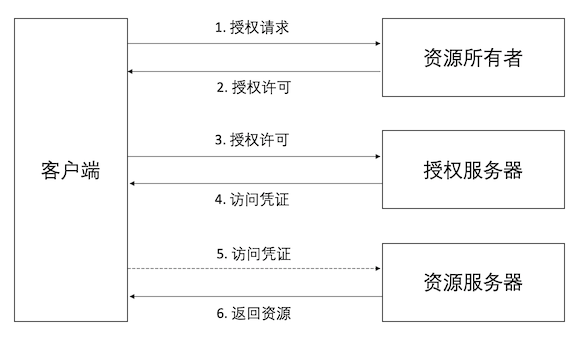
\includegraphics [width=400pt]{figures/oauth.png}
\caption{OAuth2.0协议中授权码模式的正常工作流程}
\label{fig:oauth}
\end{figure}

这里主要介绍OAuth 2.0框架中授权码模式的正常工作流程。如图\ref{fig:oauth}所示,该流程主要有以下3个阶段:

\begin{enumerate}
	\item 客户端向资源所有者发送授权请求,请求获取相应的资源访问权限。资源所有者收到请求和,检查请求的权限,通过验证后返回对应的授权许可给客户端。
	\item 客户端将授权许可发送给授权服务器,授权服务器验证后将对应资源的访问凭证返回给客户端。
	\item 客户端将访问凭证发送给资源服务器,资源服务器验证凭证后执行相应操作,并将结果返回给客户端。
\end{enumerate}


% !TeX root = ../main.tex

\chapter{区块链技术}

\section{区块链系统简介}

区块链技术旨在不可信的开放网络中,维护一个安全可信、不可篡改的公共账本,并以此为基础构建电子 交易、访问控制等应用系统.根据新节点的加入是否需要授权认证,区块链系统可以分为许可链和非许可链两 大类.非许可链通常也称为公有链,不限制节点的加入或退出,任何节点可以访问链上数据、发布交易、以及 参与链上数据的记录,甚至可以尝试发布不合法消息,攻击网络中的其他节点.许可链指区块链网络中节点 的加入网络、记录账本等操作需要经过特定的授权许可与认证.许可链系统又可以根据系统参与方的数量分 为联盟链与私有链,其中联盟链由多方组织加入同一区块链网络中,共同维护区块链账本,记录并执行链上合 约,多方组织可以通过一致的账本建立起联盟成员之间的信任.而私有链通常由一个参与方负责创建和维护, 主要用于记录和管理内部数据,增强数据的安全性、可追溯性. 

本文对比许可链和非许可链两类区块链系统在准入限制、参与方数量、采用的共识算法、应用场景等方面的区别,并总结如表\ref{tab:classification} 所示. 

\begin{table}[htb]
  \centering
  \begin{minipage}[t]{1\linewidth} % 如果想在表格中使用脚注,minipage是个不错的办法
  \caption[模板文件]{区块链系统分类}
  \label{tab:classification}
    \begin{tabularx}{\linewidth}{lXX}
      \toprule[1.5pt]
      {\heiti 名称} & {\heiti 非许可链} & {\heiti 许可链} \\\midrule[1pt]
		准入限制  & 无准入限制,任意节点可以随时加入或者退出 & 有准入限制,准入限制由整个联盟的节点商议后制定 \\
		参与方数量  & 较多 & 较少 \\  
		共识算法  & POW, POS等共识算法 & BFT类分布式共识算法 \\  
		区块链性能  & 较低 & 较少 \\  
		应用场景	 & 密码货币交易系统 & 公司间合同,公司内事务管理 \\  
		典型应用  & Bitcoin, Ethereum & HyperLedger, Coco \\
      \bottomrule[1.5pt]
    \end{tabularx}
  \end{minipage}
\end{table}

\section{密码学基础}

区块链系统中引入大量的密码学技术提供安全性、可信性等密码学性质,并以此作为区块链价值的底层保障。目前主要有哈希算法、非对称加密体制、电子签名、布尔集合、密码累加器、同态加密、零知识证明、安全多方计算等密码学技术用于区块链系统。本章主要介绍广泛应用的哈希算法,非对称加密,电子签名和布尔过滤器。

\subsection{哈希函数}

哈希函数,通常也称散列函数,是一种将任意长度的输入转换为固定长度的输出的函数。哈希函数的表示形式为:
$$h=H(m)$$
其中,m为任意长度消息,H为哈希函数,h为固定长度的哈希值,通常也称为消息摘要。

哈希函数具有如下特性:
\begin{enumerate}
\item 单向性:从输入计算输出很简单,但在不知道输入的情况下,通过输出计算出输入是计算上不可行的;
\item 输出的随机性:即算法输出的每一位数据在统计学意义上都符合随机分布;
\item 雪崩效应:对输入的任何一点修改,都会导致输出的大量变化;
\item 抗碰撞性:找到两个具有相同的输出的不同输入,是计算上不可行的。
\end{enumerate}

正是由于上述重要特性,哈希算法被广泛应用于消息认证码、随机数产生、错误校正与检测等领域,而在区块链系统中,哈希算法主要用于检查数据是否被篡改,提供工作量证明,构造存在性证明这几个用途。传统互联网中,哈希算法常用于数据的完整性验证。为了验证互联网中的文件在传输过程中是否被篡改,通常采用存储验证文件哈希值的方式,利用了哈希函数的雪崩效应和抗碰撞性,一旦数据被篡改,最终的哈希值一定与之前存储的哈希值不同。而在区块链系统中,由于交易数据不断增长,账户状态不断变化,如果采用全部数据求哈希值的方法,则每次改变都需要重新计算哈希值,计算复杂度不可接受。因此,在区块链系统中,数据根据时间顺序组织成了若干个区块,一定时间内新发生的事务数据存储在一个新区块里,每一个区块都包含了上一个区块的哈希值。这样的数据组织方式如同区块形成的链状结构,因而称为区块链。具体组织结构如图\ref{fig:hashchain}所示。


\begin{figure}
\centering	
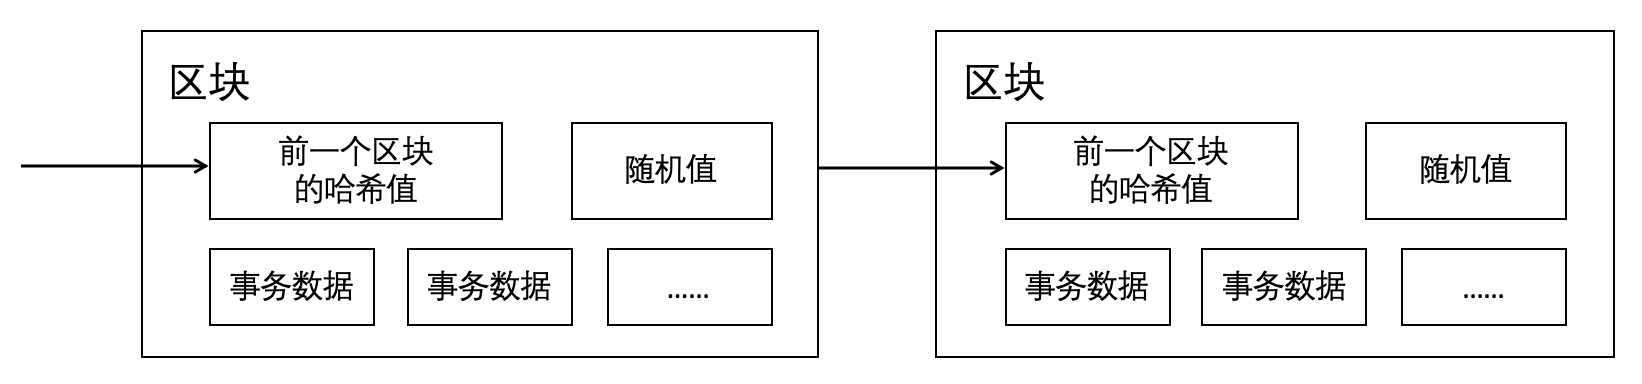
\includegraphics [width=400pt,height=100pt]{figures/hashchain.png}
\caption{区块链数据结构}
\label{fig:hashchain}
\end{figure}

如果区块链中任意区块里的数据被篡改,那么该区块的哈希值与后一区块记录的哈希值不相等。由哈希函数的雪崩效应可知,区块链上的任何历史数据改动都能被检测。因此,节点只需要存储最新区块的哈希值,即可通过计算检验历史上所有区块中的数据是否被篡改。

\begin{figure}
\centering	
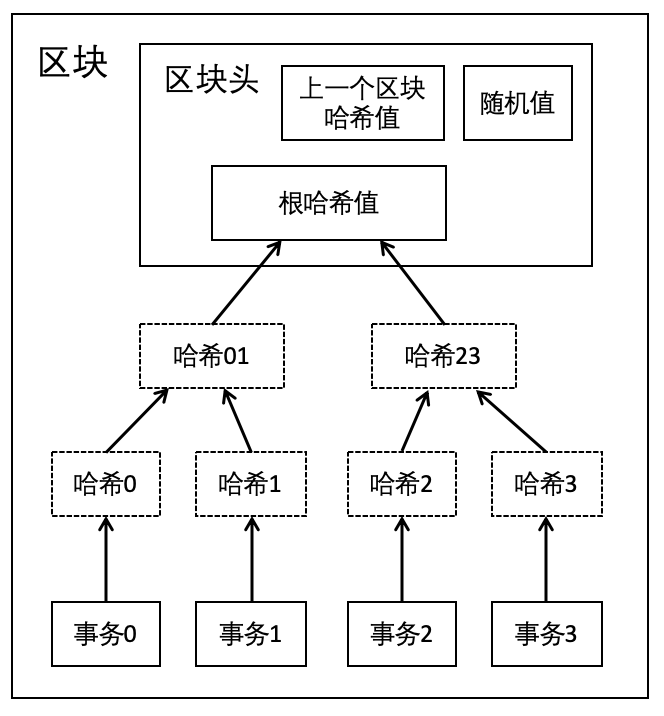
\includegraphics [width=150pt,height=180pt]{figures/merkle-tree.png}
\caption{默克尔树数据结构}
\label{fig:merkle-tree}
\end{figure}

而在每个区块中,哈希函数用于构建默克尔树,即哈希二叉树。如图\ref{fig:merkle-tree}所示,所有事务的哈希值通过二叉树结构进行哈希计算,最终计算得到根哈希值。该数据结构保证,任意事务数据的修改,都会影响到根哈希值。因此区块头中只需要存储根哈希值,就可以验证该区块中所有事务是否被篡改。


\begin{figure}
\centering	
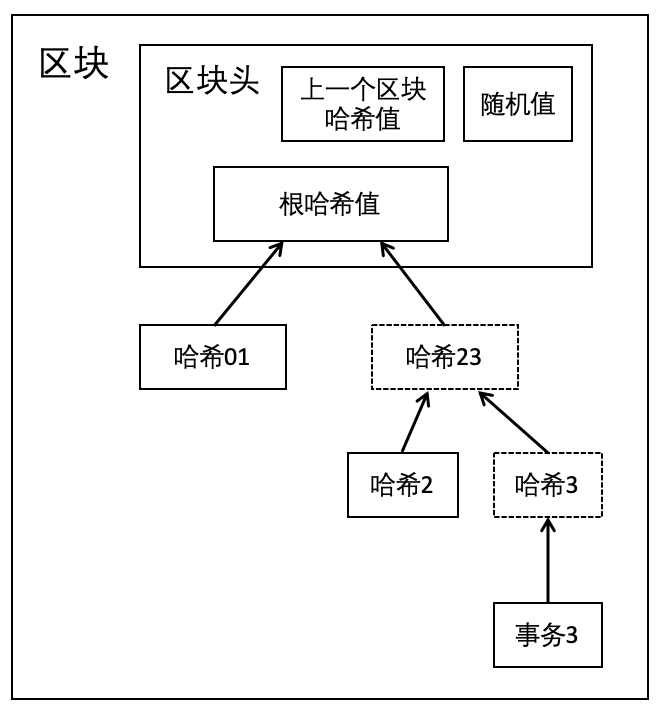
\includegraphics [width=150pt,height=180pt]{figures/merkle-proof.png}
\caption{交易存在性证明}
\label{fig:merkle-proof}
\end{figure}

当用户需要通过根哈希值验证某事务是否在某区块中时,不需要验证该区块中所有事务数据,只需要由存储所有数据的节点提供该事务到根哈希值的路径上所有相关数据。如图\ref{fig:merkle-proof}所示,当用户希望验证事务3是否存储在区块中,只需要验证“事务3”,“哈希2”,“哈希01”这几个数据是否能通过哈希函数得到根哈希值。由哈希函数的抗碰撞性可以保证,证明节点不能提供虚假数据计算出同样的根哈希值。

\subsection{非对称密码体制和电子签名}

密码体制主要分为对称密码体制和非对称密码体制。简单来说,对称密码体制指加密算法中使用的加密密钥和解密算法中使用的解密密钥是相同的密钥,或者解密密钥能通过加密密钥计算得到。而非对称密码体制中,这两者不同,并且解密密钥不能通过加密密钥计算得到。

\begin{figure}
\centering	
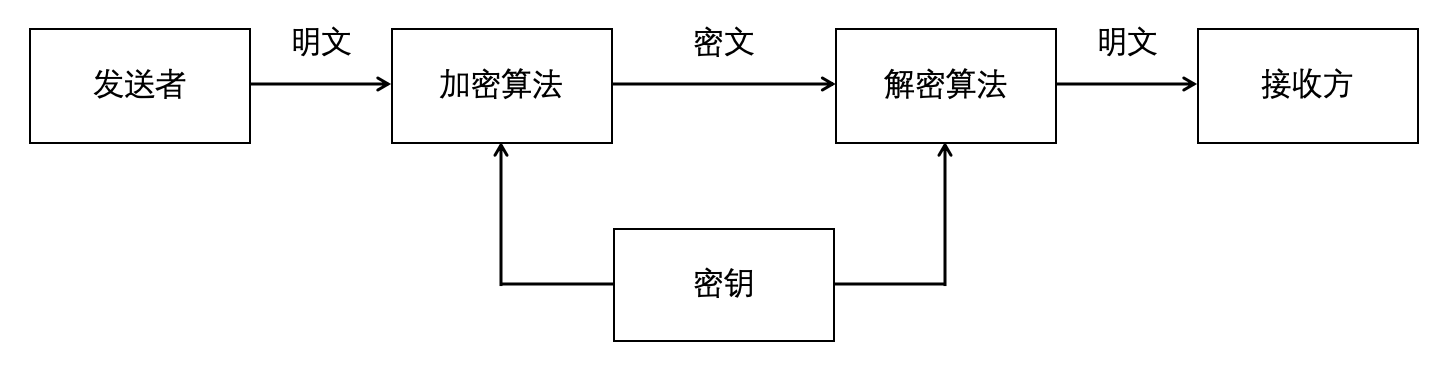
\includegraphics [width=400pt,height=100pt]{figures/sym-crypto.png}
\caption{对称密码体制的基本模型}
\label{fig:sym-crypto}
\end{figure}

如图\ref{fig:sym-crypto}所示,对称密码体制中,发送者先使用密钥和加密算法将明文加密为密文,然后传输密文给接收方,接收方使用解密算法和相同的密钥将密文解密回原始的明文。因为加密和解密算法使用的密钥需要相同,消息发送方和接收方必须在密文传输前通过安全信道进行密钥传输。因此对称密码体制面临密钥分配问题,目前主要通过通信双方直接进行密钥传输或者密钥分配中心进行密钥分发进行。然而实际的传输信道安全性并不理想,密钥在传输过程中被暴露的风险很大,增加了系统的脆弱性。另一方面,在有多个用户的网络中,任何两个用户之间都需要共享加密密钥。当网络中用户$n$很大时,需要管理的密钥数目为$C_n^2$,复杂度近似O($n^2$)。当有一个新用户加入时,需要产生$n$个秘密的密钥,并秘密分发给$n$个用户。对称密码体制中使用的加密算法主要采用扩散和混淆两种基本方法,可以抵抗密码分析技术对密文进行统计分析。扩散指让明文中的每一位尽可能多影响密文中的若干位,以及让密文中的每一位受到明文中尽可能多位的影响,这样可以隐蔽明文的统计特性。字符到字符的映射,通常包含单字符置换和多字符置换。混淆指混淆密文与密钥之间的统计关系,使得对手即使获取了关于密文的一些统计特性,也无法推测密钥。通常使用复杂的非线性代替变换可以达到比较好的混淆效果。

\begin{figure}
\centering	
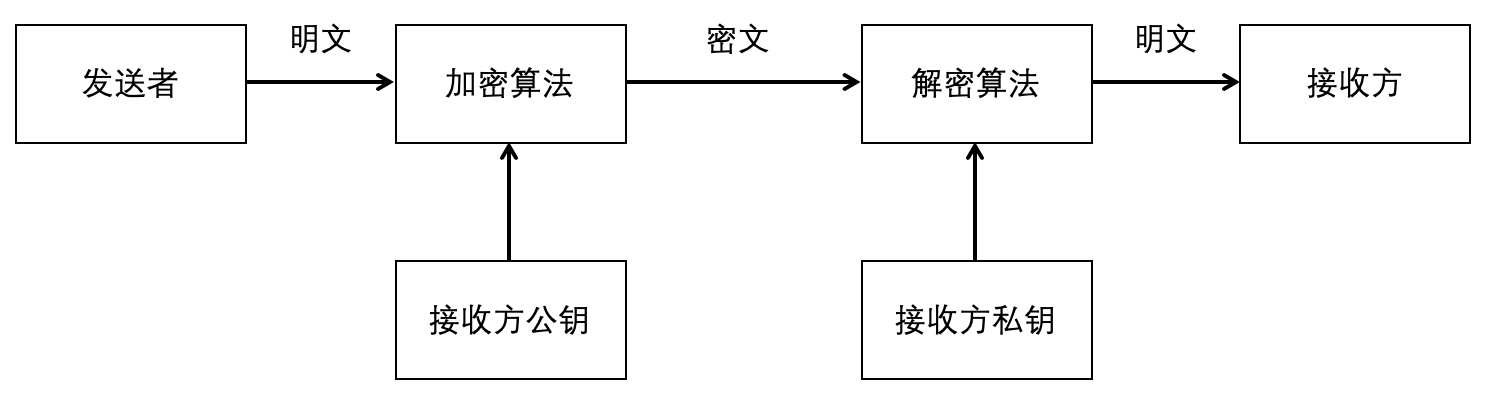
\includegraphics [width=400pt,height=115pt]{figures/asym-crypto.png}
\caption{非对称密码体制的基本模型}
\label{fig:asym-crypto}
\end{figure}

1976年,W.Diffie和M.Hellman在IEEE Trans.on Information刊物上发表了“ New Direction in Cryptography”文章,提出了“非对称密码体制“的概念,开创了密码学研究的新方向。如图\ref{fig:asym-crypto}所示,非对称密码体制中,密钥分为成对的加密密钥和解密密钥,其中加密密钥公开,解密密钥保密。公开的密钥可以作为用户的个人身份,由公开的加密密钥无法推导相应的解密密钥。因此即使将加密密钥公开也不会暴露解密密钥,不会损害密码的安全。因此,通信双方可以通过不安全的信道交换公钥,然后用对方的公钥对消息进行加密并传输,达到在不安全的信道上保密传输的效果。解决了对称密码体制中需要安全信道的问题,同时在密钥管理上也极大降低了网络中需要管理的密钥数量,从对称密码体制的$C_n^2$降低到$n$。对称密码体制与非对称密码体制在密钥分发、密钥管理等方面的区别主要如表\ref{tab:sym-asym}所示。

\begin{table}[htb]
  \centering
  \begin{minipage}[t]{1\linewidth}
  \caption{对称密码体制与非对称密码体制的区别}
  \label{tab:sym-asym}
    \begin{tabularx}{\linewidth}{lXX}
      \toprule[1.5pt]
      {\heiti 功能} & {\heiti 对称密码体制} & {\heiti 非对称密码体制} \\\midrule[1pt]
		密钥分发  & 需要事先进行安全的密钥分发 & 不需要事先进行安全的密钥分发,公钥可以在不安全的信道上传输 \\
		密钥管理  & 每个用户需要保存n个不同密钥用于与其他n个用户通信。当有新用户加入时,每个用户都需要和新用户共享一个新密钥,整个系统中需要存储O($n^2$)个密钥 & 每个用户只需要存储自己的公钥和私钥,整个系统中只需要存储O(n)个密钥 \\
		电子签名  & 不支持电子签名功能 & 支持电子签名功能 \\  
		性能  & 加密算法和解密算法简单,加解密速度较快 & 加密算法和解密算法需要进行复杂的数学运算,速度较慢 \\  
		安全性  & 安全性来源于混淆和置换 & 安全性通常基于数学难问题,部分假设未证明 \\ 
      \bottomrule[1.5pt]
    \end{tabularx}
  \end{minipage}
\end{table}

数字签名,通常也称为电子签名,指通过数据处理的方式对数字消息进行签名。同样具有手写签名的两大特性:可验证性和防伪造性。具体来说,数字签名需要具备以下特性:

\begin{enumerate}
 \item 任何人可以验证数字签名是否由消息的发送方生成。
 \item 任何人不能伪造发送方的数字签名,这也意味着发送方不能抵赖自己生成的数字签名。
 \item 任何人可以验证数字签名是否匹配发送的消息,因此可以验证消息从发送到接受过程中是否被篡改。对整个消息生成数字签名过于复杂,因此通常先对消息计算哈希值,然后生成哈希值的数字签名用于验证。
\end{enumerate}

某种意义上,我们可以认为数字签名的过程是一种加密,而对签名还原到原消息,然后进行验证是一种解密。但与非对称公钥体系中的公钥加密,私钥解密恰好相反,通过私钥计算签名,然通过公钥进行验证。由于公钥公开,因此所有人可以知道该公钥的持有者。而只有该用户拥有对应的私钥,才能生成正确的数字签名。

在区块链领域,每个用户都可以通过特定算法独立生成任意多账户,即公私钥对。当用户发起事务时,需要用私钥生成事务数据的电子签名。当该事务涉及其他用户时,使用特定用户公钥生成的地址。

\subsection{布尔过滤器}

为了验证某数据是否存在集合中,传统算法主要有遍历查找,二分查找,索引查找等,这些算法的时间消耗都会随着集合数量的增加而增加。为了解决这一问题,布尔过滤器利用哈希算法的输出长度固定性和随机性,利用固定长度的数组存储集合,对元素进行哈希变换,然后根据输出找到对应下标并在数组中记录或查询。为了解决不同输入映射到同一下标的问题,通常采用多个哈希函数共同确认。布尔过滤器具有很好的空间和时间效率,被用来检测一个元素是不是集合中的一个成员。在以太坊项目中,布尔过滤器被用于检测交易是否在给定区块中,便于用户快速检索特定交易的存储位置。和布尔过滤器类似,密码累加器也用于高效验证数据的存在性,后者还可以提供高效安全的存在性证明。在零币项目中,密码累加器用于存储用户加入的未花费代币的对应编码,当用户使用时,其他用户可以高效验证花费的代币是否存在。

\section{共识协议}

\subsection{传统分布式共识协议}
\label{subsec:traditional-consensus}

PAXOS

RAFT

PBFT

\subsection{工作量证明共识协议}
\label{subsec:work-proof}

在区块链领域,尤其在公有链网络中,节点可以自由加入或退出网络,因此无法采用基于身份投票的方式。传统的分布式共识算法无法使用。因此在公有链领域广泛使用比特币系统提出的工作量证明共识算法及其变形。

首先我们介绍比特币系统提出的工作量证明算法,工作量证明最早用于抵抗针对邮件服务器的拒绝服务攻击以及防止垃圾邮件的发送。

为了解决比特币系统的性能瓶颈,以太坊项目提出了GHOST协议,该协议将最长链共识原则改为最大子树共识原则。

而以太坊提出的最大子树共识只利用了分叉块的工作量,为了进一步提升系统性能,conflux协议在此基础上进一步利用了分叉块中未冲突的交易。



% !TeX root = ../main.tex

\chapter{基于属性的访问控制系统}

\section{系统框架}

\begin{figure}
\centering
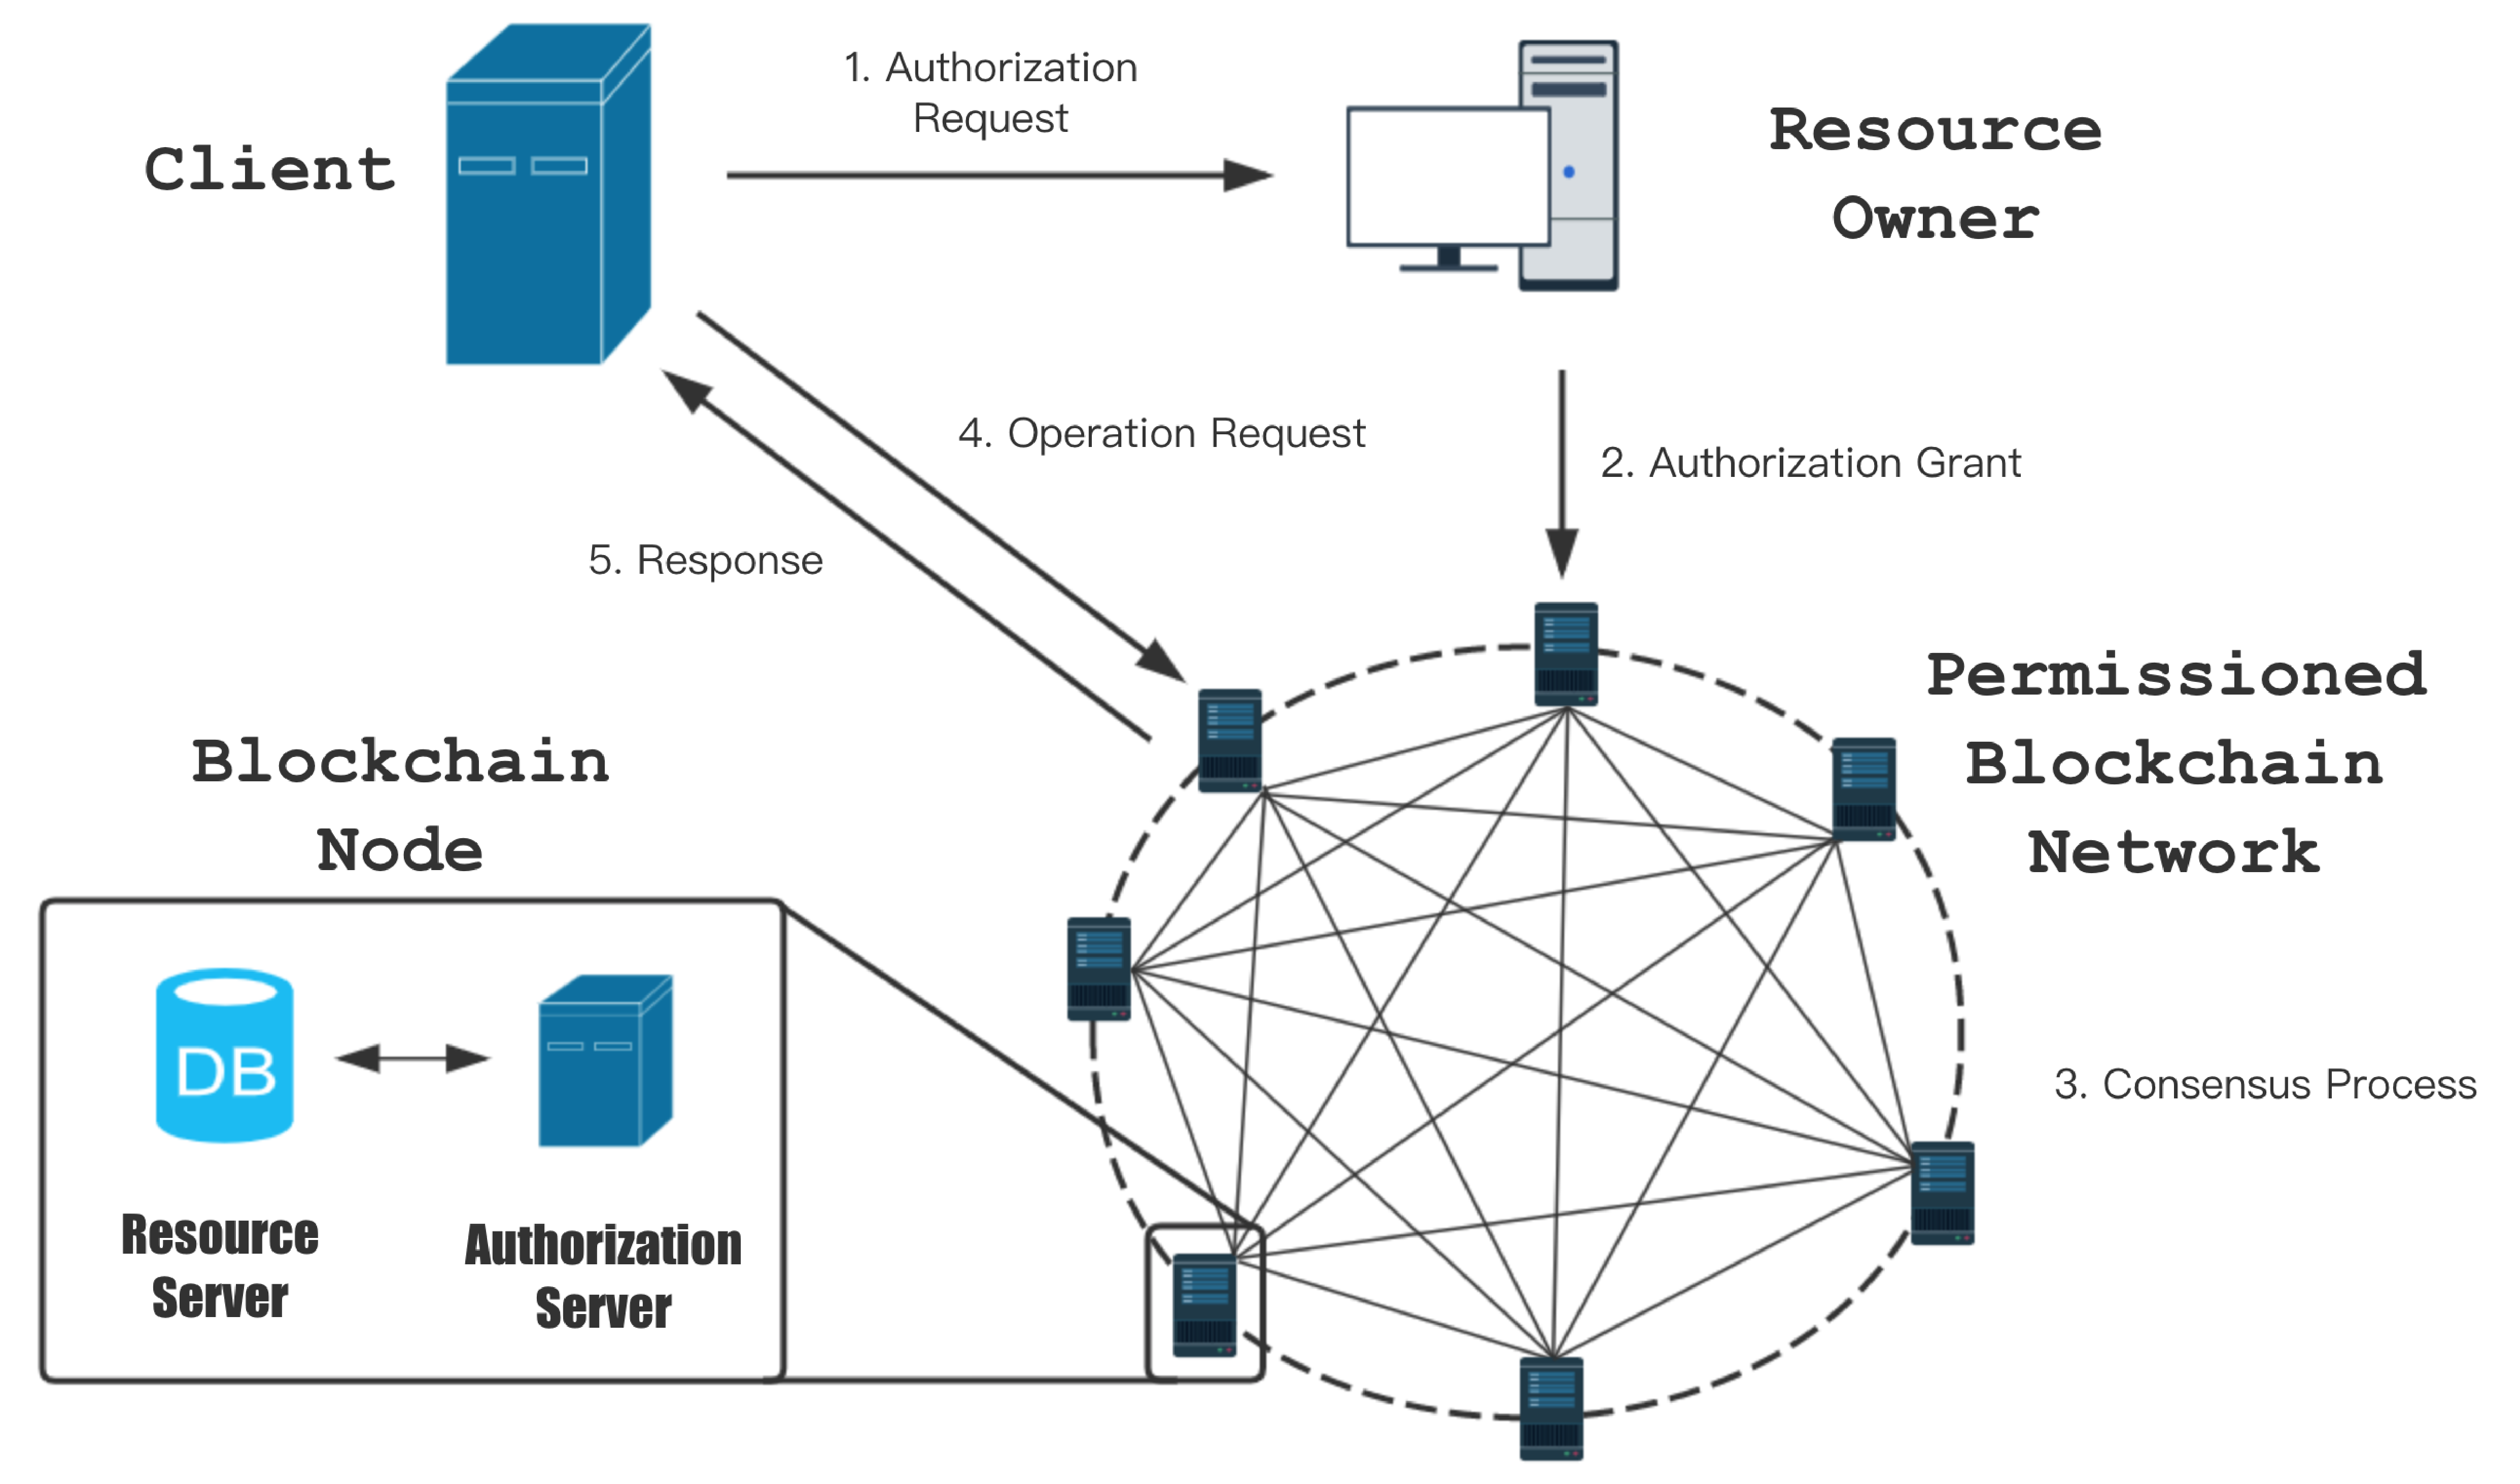
\includegraphics[width=11cm]{figures/archi.eps}
\caption{The Architecture of Decentralized Authorization and Authentication}
\label{fig:framework}
\end{figure}

通过运用区块链技术和基于属性的访问控制模型,我们提出了一个联盟链架构,类似OAuth框架用于第三方授权和认证。图\ref{fig:framework}给出了架构设计和工作流程的概述。该系统包含三类角色,“客户端”作为资源请求者,它请求资源所有者进行授权,并最终请求区块链节点访问资源。“资源所有者”在区块链节点上存储资源,在需要时授予“客户端”访问受保护资源的权限。该架构以联盟网络代替OAuth框架中的中心化认证服务器和资源服务器,该网络中的每个节点具有平等的地位,各自存储用户特定资源并且共同参与用户数据授权和身份验证数据的存储和管理。每个节点由资源服务器和授权服务器组成,其中资源服务器存储用户资源并使用基于属性的访问控制策略进行认证管理。当接收到操作请求时,资源服务器可以使用访问控制策略列表对请求中的各项属性进行身份验证。授权服务器与其他节点的授权服务器共同管理区块链,将用户发起的授权数据存储在区块链中,并且它可以根据区块链对资源服务器提供用于身份验证的各账户的主体属性。

\begin{description}
  \item[\textbf{资源所有者}] 资源所有者存储自己的资源在资源服务器,并在需要时授予客户端访问受保护资源的权限。
  \item[\textbf{客户端}] 客户端指资源请求者,通过向资源所有者发送请求获取授权,并访问资源服务器获取资源。不同于OAuth框架中客户端需要提前注册,任何用户都可以独自创建账户作为客户端。
  \item[\textbf{区块链节点}] 联盟链网络由若干互联的区块链节点组成。每个节点包含授权服务器和资源服务器。其中资源服务器保管资源所有者存储的部分资源,并采用基于属性的访问控制模型验证操作请求。所有节点的授权服务器共同运行共识协议,管理记录资源所有者对客户端的授权,并维护账户的属性状态。
\end{description}

该系统在以下几个方面提高了OAuth等中心化访问控制架构的安全性:

\begin{enumerate}
  \item OAuth框架中,第三方平台需要事先在授权服务器进行注册获取客户端密码,然后将客户端密码发送到授权服务器验证身份并获取访问令牌。一旦攻击者入侵了中心化的授权服务器,就可以通过发布伪造的令牌,从而伪装成任何用户访问资源服务器中受保护的资源。该系统中采用的非对称加密系统和去中心化架构可以有效降低攻击的严重程度。在共识达成一致的联盟网络中,攻击者只能访问被入侵的服务器中存储的资源。由于用于电子签名的私钥由用户本地生成并保管,用户发起的操作和授权不能被伪造,从而保护了存储在其他平台上的资源。

  \item 系统中使用的数字签名可以防止跨站请求伪造(Cross-Site Request Forgery,CSRF)攻击。OAuth框架在多个平台广泛实现,并使用重定向URL连接不同的平台,这可能会带来CSRF攻击。例如,它通常用于中心化平台和第三方平台之间的帐户绑定。攻击者可以先访问授权服务器,获得绑定第三方平台和中心化平台账户的访问令牌,然后诱使用户向第三方平台发送绑定请求,并提前提供攻击者获得的令牌。因此,攻击者可以通过中心化平台的账号访问第三方平台上的用户资源。在我们的系统中,用户发送的所有授权和操作都需要进行数字签名,这样才能保证授权的来源。
\end{enumerate}

\section{协议流程}
\label{sec:protocols}
本节介绍此框架中的协议。整个协议主要分为5个步骤,分别对应于图\ref{fig:framework}中的工作流程。每一步的详细信息在\ref{sec:protocols}中描述,具体步骤如下:

\begin{enumerate}
  \item 客户端向资源所有者发送$Authorization Request$,其中主要包含客户端的地址和请求授权的属性。
  \item 资源所有者检查$Authorization Request$,如果同意则生成相应的$Authorization Grant$并且发送给任何区块链节点。
  \item 如果接收到的$Authorization Grant$有效,则区块链节点将接受并在网络中传播它。共识过程结束后,授权将被打包到一个新的区块中,并记录到区块链上。
  \item 获得授权后,客户端找到存储需要访问资源的区块链节点,并发送$Operation Request$给该节点的资源服务器。
  \item 资源服务器根据授权服务器提供区块链上账户的主体属性,存储的资源属性以及基于属性的访问控制策略来验证$Operation Request$,根据验证结果回应客户端。
\end{enumerate}

接下来将详细介绍各步骤的细节。首先介绍后续涉及的一些密码学表示,对于消息$m$,我们定义$H(m)$表示$m$的哈希值,并且用$\langle m \rangle_{\sigma_{i}}$ 表示消息 $m$ 以及节点$i$对 $H(m)$ 的签名。可以用于验证该消息的真实来源以及是否在传输中被篡改。

\subsection{区块链和属性状态}

该系统中,区块链是用来存储授权记录的基本数据结构,每个区块记录一系列授权信息,每个授权信息包括发送方地址,接收方地址,授权属性,授权有效期以及用于验证的签名等信息。为了在本系统中,我们采用了以太坊项目中的账户状态机制,而非比特币项目中的未花费输出(Unspent Transaction Output, UTXO)机制,因为状态设计更适合ABAC模型。我们将账户中的余额等信息修改为属性状态,区块链记录每个账户拥有的所有属性以及nonce值,每个属性包括属性名和有效期。全局状态指所有帐户的信息。根据区块链,我们可以计算包含地址、nonce和属于地址的属性状态的每个帐户的状态。状态保存在内存中,可用于验证授权或操作。在区块链上添加新块时,全局状态将根据新块中的授权进行更改。我们可以将全局状态视为区块链的当前结果。对于帐户状态中的nonce值,每个帐户都有一个nonce值,其值为0。地址D的一次授权记录在区块链上时,地址D的一次授权将增加1。任何与nonce值不匹配的授权都将被拒绝。这可以防止重播攻击,因为一旦在区块链上记录了授权,就不能再接受它,因为增加了nonce值。

\subsubsection{对授权的验证}

联盟链网络中的节点收到客户端发送的授权后,首先验证该授权,如果通过则添加到授权池中,等待打包进新区块。更多细节在算法 \ref{alg:authVerify}中介绍。

 \begin{algorithm}
 \floatname{algorithm}{Algorithm}
 \caption{授权验证}\label{alg:authVerify}
   \begin{algorithmic}[!htbp]
   \renewcommand{\algorithmicrequire}{\textbf{Input:}}
   \renewcommand{\algorithmicensure}{\textbf{Output:}}
   \REQUIRE $Authorization$
   \ENSURE  $Verification$
    \STATE $Sender$, $Receiptor$, $Attributes$, $nonce$, $Signature \gets Parse(Authorization)$
    \STATE $AuthorizationHash \gets Hash(Authorizaton)$
    \IF {$CheckSignature(Sender, Hash, Signature) \ne true$}
      \RETURN $false$
    \ENDIF
    \STATE $SenderState \gets GetStateFromAddress(Sender)$
    \IF {$nonce < SenderState.nonce$}
      \RETURN $false$
    \ENDIF
    \FOR {$each Attribute \in Attributes$}
      \IF {$SenderState.VerifyAttribute(Attribute) \ne true$}
        \RETURN $false$
      \ENDIF
    \ENDFOR
    \STATE AddAuthorizationToPool(Authorization)
   \RETURN $true$
   \end{algorithmic}
 \end{algorithm}

\subsubsection{对操作请求的验证}

资源服务器能获取同一节点中授权服务器同步的区块链状态,因此,当收到客户端对资源的操作请求时,资源服务器首先通过授权服务器获取客户端地址拥有的属性,即主体属性,然后获取被访问资源对应的客体属性,操作请求对应的操作属性,以及当前的环境属性(即时间戳)。最后根据自己存储的属性访问控制列表对所有属性进行计算得到是否允许该操作。具体过程如算法 \ref{alg:opVerify}所示.

 \begin{algorithm}
 \floatname{algorithm}{Algorithm}
 \caption{验证操作}
   \begin{algorithmic}[H]\label{alg:opVerify}
   \renewcommand{\algorithmicrequire}{\textbf{Input:}}
   \renewcommand{\algorithmicensure}{\textbf{Output:}}
   \REQUIRE $Operation$
   \ENSURE  $Verification$
    \STATE $Sender$, $OpCode$, $Obj$, $nonce$, $Timestamp$, $Signature \gets Parse(Operation)$
    \STATE $OperationHash \gets Hash(Operation)$
    \IF {$CheckSignature(Sender, Hash, Signature) \ne true$}
      \RETURN $false$
    \ENDIF
    \STATE $SenderState \gets GetStateFromAddress(Sender)$
    \IF {$nonce < SenderState.nonce$}
      \RETURN $false$
    \ENDIF
    \STATE$SubAttributes \gets GetAttrFromAddress(Sender)$
    \STATE$ObjAttributes \gets GetAttrFromObject(Obj)$
    \STATE$OpAttributes \gets GetAttrFromOpCode(OpCode)$
    \STATE$EnvAttributes \gets Timestamp$
    \FOR {$each Policy \in Policies do$}
      \IF {$Policy.Match$($SubAttributes$, $ObjAttributes$, $OpAttributes$, $EnvAttributes$) = $true$}
        \RETURN $true$
      \ENDIF
    \ENDFOR
   \RETURN $false$
   \end{algorithmic}
 \end{algorithm}

\subsubsection{区块生成算法}

联盟网络中的节点会将一段时间内接受到的授权信息打包到一个新区块中,在比特币系统中这个时间间隔是10分钟,而在以太坊中是15秒,动态调整的具体方法在前文章节\ref{subsec:work-proof}中有所介绍。而在本系统中,为了保障访问控制系统的延迟可接受,我们设置区块间隔为2秒,区块生成的具体算法在算法\ref{alg:blockGeneration}中介绍。

 \begin{algorithm}
 \floatname{algorithm}{Algorithm}{}
 \caption{Block Generation}\label{alg:blockGeneration}
   \begin{algorithmic}[!htbp]
   \renewcommand{\algorithmicrequire}{\textbf{Input:}}
   \renewcommand{\algorithmicensure}{\textbf{Output:}}
   \REQUIRE $AuthorizationPool, AUTH\_LIMIT, PreviousBlock$
   \ENSURE  $Verification$
    \STATE $auths \gets ChooseAuths(AuthorizationPool, AUTH\_LIMIT)$
    \STATE $prevHash \gets H(PreviousBlock)$
    \STATE $timestamps \gets CurrentTime()$
    \STATE $newBlock \gets NewBlock(prevHash, auths, timestamps)$
   \RETURN $newBlock$
   \end{algorithmic}
 \end{algorithm}

\subsection{改进的PBFT共识算法}

在前文第\ref{subsec:traditional-consensus}节中,我们介绍了多种一致性算法,用于保证分布式节点间数据的一致性,其中拜占庭容错算法能提供拜占庭式容错(BFT)。实用的拜占庭容错算法(PBFT)于1999年提出,减少了BFT的时间和通信复杂度,并已应用于区块链领域的超级账本项目中。我们在访问控制系统中采用了改进的PBFT算法。区块链网络广播中的节点向其他节点发送请求。经过一段时间后,主节点将合法请求打包成块。然后将该块广播到网络中,与其他节点取得一致的结果。

\subsubsection{节点和视图}

主节点、备份节点和视图更改基本采用PBFT算法的设计。但存在如下差异,PBFT算法中的主节点在接收到来自客户端的请求时开始协商过程。在这个系统中,主节点每2秒启动一次协商,并将最多1000个授权打包到一个新区块中。当备份节点发现主节点似乎发生故障或被攻击时,将发生视图更改,这与PBFT算法中的视图变化相同。除此之外,当一段时间后,系统中的节点也会自动进行视图更改。这可以防止来自恶意主节点的黑名单攻击。在区块链系统中,生成新块的节点可以选择其中包含的事务以及先后顺序,恶意节点可以拒绝打包黑名单中帐户的事务。因此,不断的视图更改可以防止来自恶意主节点的黑名单攻击。

\subsubsection{预准备阶段}

当一个新区块过程开始,所有节点进入预准备阶段。这一阶段中,主节点从授权池中选择一系列合法的授权,并且打包到一个新区块中。然后,主节点广播预准备信息$\langle PRE$-$PREPARE, v, i, block \rangle_{\sigma_{i}}$ 给所有备份节点,其中 $v$ 表示当前的视图编号,$i$ 表示主节点的节点编号。具体预准备信息$pre$-$prepare$的创建如算法\ref{alg:preprepareGen}所示。

 \begin{algorithm}
 \floatname{algorithm}{Algorithm}
 \caption{生成预准备信息}\label{alg:preprepareGen}
   \begin{algorithmic}[H]
   \renewcommand{\algorithmicrequire}{\textbf{Input:}}
   \renewcommand{\algorithmicensure}{\textbf{Output:}}
   \REQUIRE $blockchain, authorizationPool, AUTH\_LIMIT,$ $sk, viewID$
   \ENSURE  $pre$-$prepare$
    \STATE $prevBlock \gets blockchain.LastBlock()$
    \STATE $block$ $\gets$ $BlockGenration(prevBlock, AUTH\_LIMIT,$ $authorizationPool)$
    \STATE $pre$-$prepare \gets NewRequest(viewID, block)$
    \STATE $signature \gets sk.Sign(request)$
    \STATE $pre$-$prepare.Signature \gets signature$
   \RETURN $pre$-$prepare$
   \end{algorithmic}
 \end{algorithm}


当备份节点接受到主节点发送的预准备信息$pre$-$prepare$后,验证过程如算法\ref{alg:prepreVerify}所示。如果通过验证,备份节点将接受该信息并进入准备阶段。否则,该节点可以认为主节点被恶意控制或者宕机,将会发起视图切换,请求选举出下一个正常节点作为新的主节点。

 \begin{algorithm}
 \floatname{algorithm}{Algorithm}
 \caption{验证预准备信息}
   \begin{algorithmic}[H]\label{alg:prepreVerify}
   \renewcommand{\algorithmicrequire}{\textbf{Input:}}
   \renewcommand{\algorithmicensure}{\textbf{Output:}}
   \REQUIRE $pre$-$prepare$, $N$, $ViewID$, $i$, $PkList$
   \ENSURE  $Verification$
    \STATE $viewID$, $nodeID$, $timestamps$, $signature \gets Parse(pre$-$prepare)$
    \IF {$viewID \ne ViewID$}
      \RETURN $false$
    \ENDIF

    \IF {$nodeID \ne ViewID \% N$}
      \RETURN $false$
    \ENDIF

    \STATE $hash \gets H(pre$-$prepare)$
    \IF {$CheckSignature(PkList[i], hash, signature) \ne true$}
      \RETURN $false$
    \ENDIF
   \RETURN $true$
   \end{algorithmic}
 \end{algorithm}

\subsubsection{准备阶段}

如果备份节点 $i$ 接受了预准备信息$pre$-$prepare$,该节点进入准备阶段。节点$i$生成准备信息$\langle PRE$-$PARE, v, i, blockHash\rangle_{\sigma_{i}}$,其中视图编号$v$和预准备信息中的视图编号一致,$i$ 表示该备份节点的节点编号,$blockHash$ 表示预准备信息$pre$-$prepare$中包含区块的哈希值。具体细节在算法\ref{alg:prepareGen}中介绍。然后该备份节点将生成的准备信息 $prepare$广播给其他所有节点,包括主节点在内。一旦某个节点从不同的来源节点(包括自己)接收到$2f+1$个拥有相同$v$和 $blockHash$的准备信息,该节点将会进入承诺阶段。

 \begin{algorithm}
 \floatname{algorithm}{Algorithm}
 \caption{生成准备信息}
   \begin{algorithmic}[H]\label{alg:prepareGen}
   \renewcommand{\algorithmicrequire}{\textbf{Input:}}
   \renewcommand{\algorithmicensure}{\textbf{Output:}}
   \REQUIRE $pre$-$prepare, nodeID, sk, NeighborList$
   \ENSURE  $prepare$

    \STATE $blockHash$ $\gets$ $H(pre$-$prepare.Block)$

    \STATE $viewID \gets pre$-$prepare.ViewID$
    \STATE $prepare \gets NewPrepare(viewID, nodeID, blockHash)$
    \STATE $signature \gets sk.Sign(prepare)$
    \STATE $prepare.Signature \gets signature$
   \RETURN $prepare$
   \end{algorithmic}
 \end{algorithm}

\subsubsection{承诺阶段}

进入承诺阶段的节点获知网络中大部分正常节点(至少f+1个)已经接受该信息。节点$i$将生成并广播承诺信息$\langle COMMIT, v, i, blockHash \rangle_{\sigma_{i}}$ 给所有节点,表明该节点将接受这一新区块作为共识结果。承诺的生成过程如算法\ref{alg:commitGen}所示。

 \begin{algorithm}
 \floatname{algorithm}{Algorithm}
 \caption{Commit Generation}
   \begin{algorithmic}[H]\label{alg:commitGen}
   \renewcommand{\algorithmicrequire}{\textbf{Input:}}
   \renewcommand{\algorithmicensure}{\textbf{Output:}}
   \REQUIRE $prepare, nodeID, blockHash, sk$
   \ENSURE  $commit$

    \STATE $viewID \gets prepare.ViewID$
    \STATE $blockHash \gets prepare.blockHash$
    \STATE $commit \gets NewCommit(viewID, nodeID, blockHash)$
    \STATE $signature \gets sk.Sign(prepare)$
    \STATE $commit.Signature \gets signature$
   \RETURN $commit$
   \end{algorithmic}
 \end{algorithm}

当某个节点从不同来源节点接收到 $2f+1$个合法的承诺信息,该节点可以确认该新区块至少被$f+1$个正常节点接受,因为在接收的$2f+1$个承诺信息中,至多只有$f$个来源于拜占庭节点。然后该节点可以将该区块记录在区块链上,并更新账户状态。

\section{原型实现}

\begin{figure}
\centering
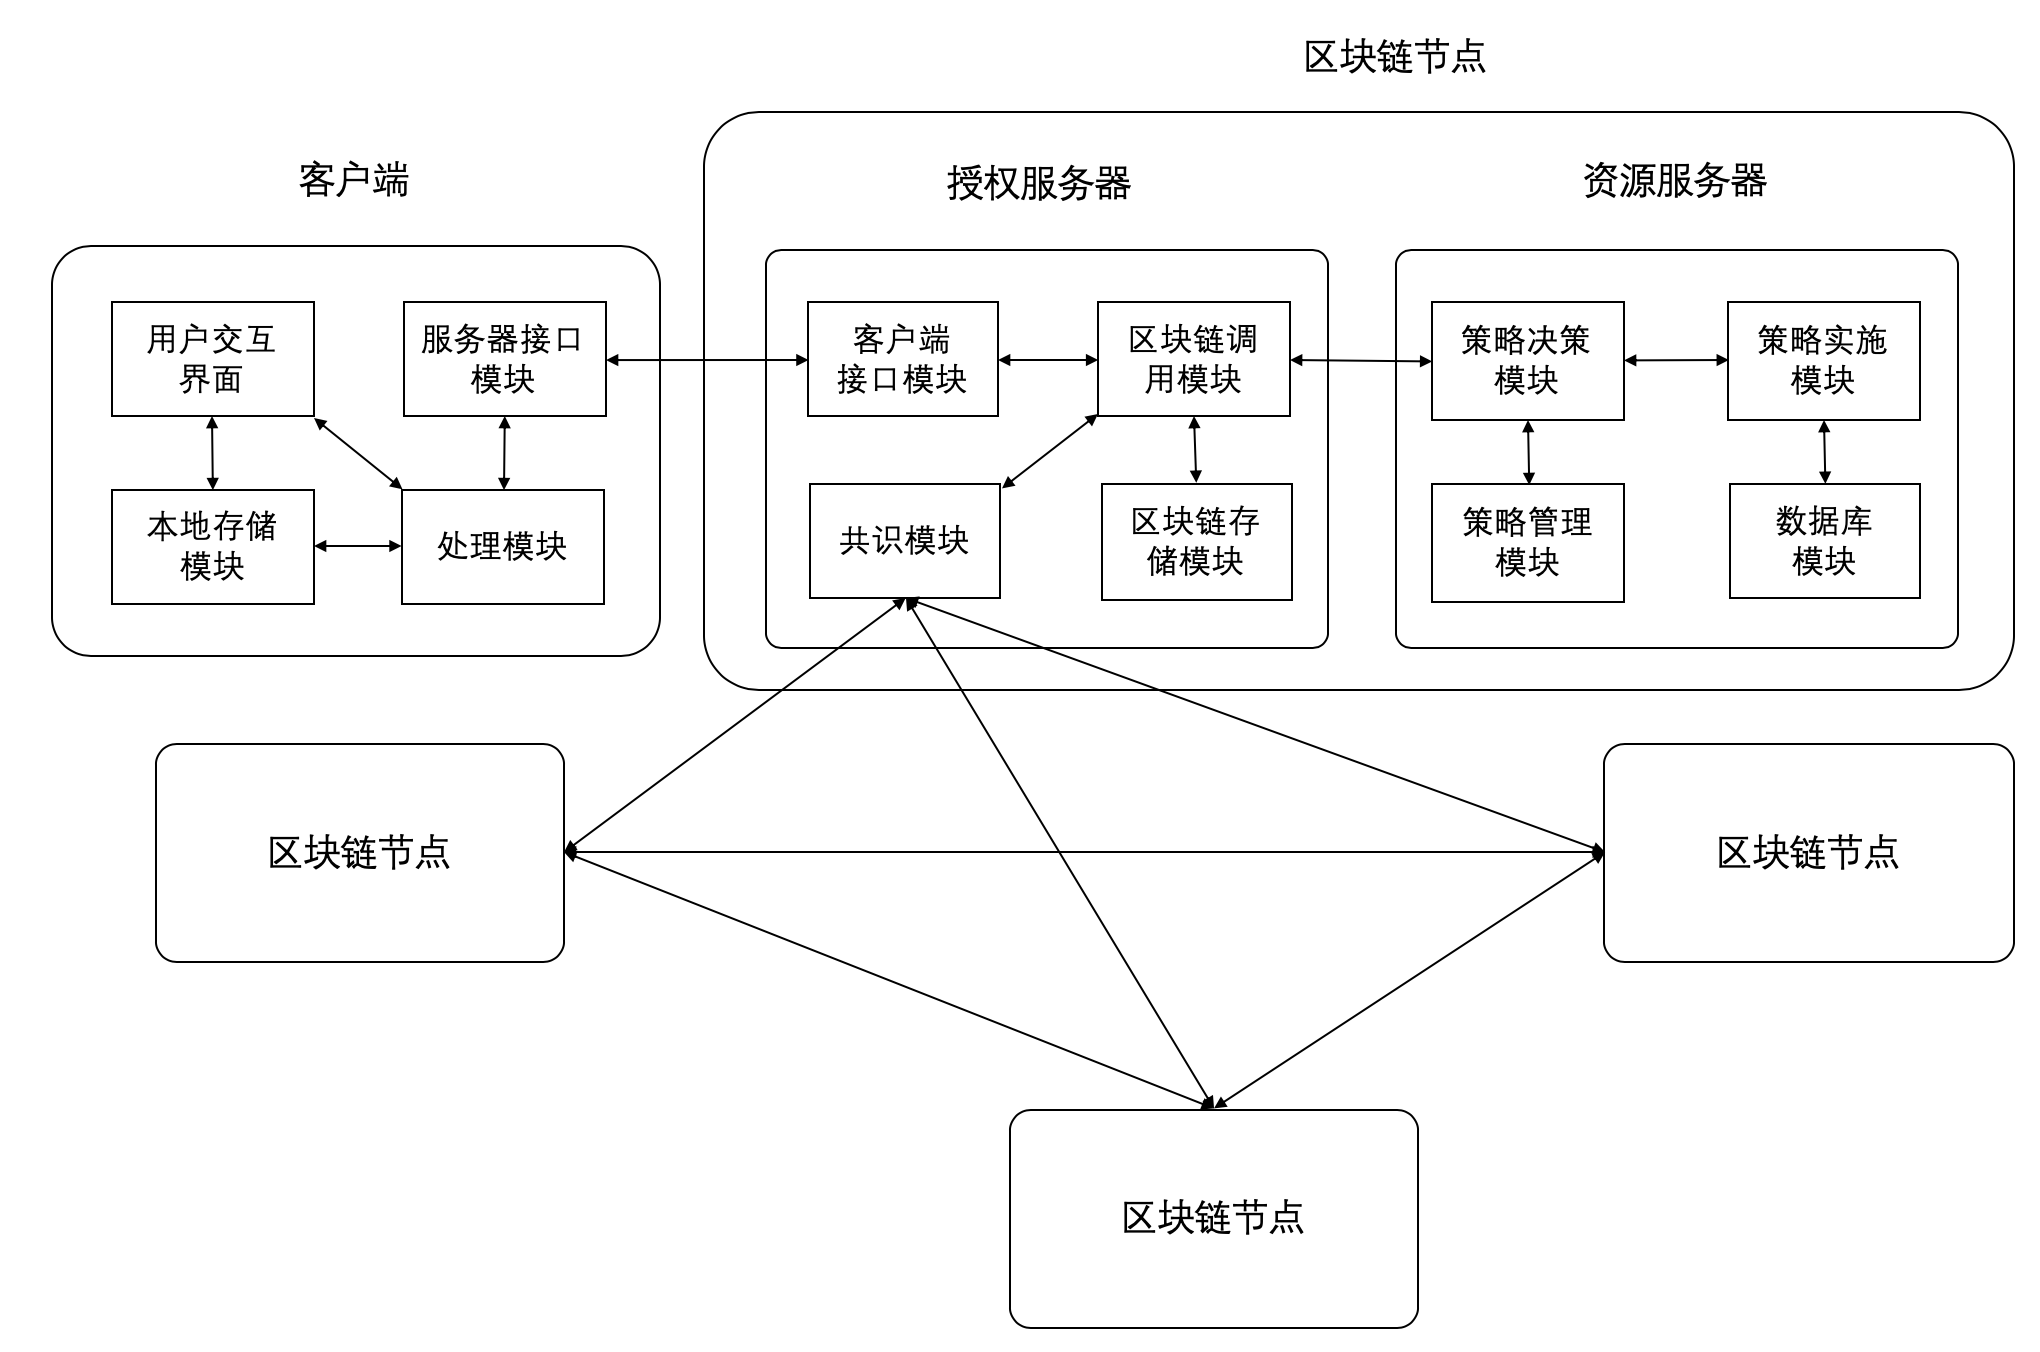
\includegraphics[width=12cm, keepaspectratio]{figures/implementation.png}
\caption{The Implementation of Prototype}
\label{fig:implementation}
\end{figure}

如图\ref{fig:implementation}所示,基于上述协议,我们实现了一个原型系统用于验证设计框架和协议的可行性,并且评估性能和延迟等重要指标。

这一系统采用Go程序语言实现,因为Go语言的并发机制(goroutines和channel通信)帮助构建高性能的网络应用,能提升访问控制系统的性能。为了简化实现,资源服务器采用键值对数据库leveldb存储资源,实际上可以采用现有的任意数据库实现。在区块链网络中,节点间的通信采用HTTP协议实现,未来还可以考虑采用UDP协议提升性能。

\begin{itemize}
  \item 客户端:与框架中客户端角色不同,这里实现的客户端用于用户管理自己的账户和密钥,授权其他用户,以及操作可访问的资源。该客户端可以生成并签名授权请求和操作请求,并且和服务器节点进行交互。
  \item 授权服务器: 授权服务器主要实现以下四个模块功能:
    \begin{enumerate}
      \item 与客户端交互模块:该模块接受客户端的授权请求和操作请求并转发给处理器模块。
      \item 区块链模块:该模块与其他服务器进行通信,发送并接受区块链相关信息,包括授权请求,区块数据等。同时负责区块数据以及状态数据的存储和更新。
      \item 共识模块:该模块发送并接受改进的PBFT协议中的相关消息,包括预准备信息,准备信息,承诺信息,更新视图等。采用多个定时器通过管道实现,保障在限定时间内达成共识产生新区块。
      \item 处理器模块:该模块处理从客户端或者其他节点接收到的消息,运行前文介绍的区块生成和验证算法。
    \end{enumerate}
  \item 资源服务器:资源服务器主要由以下两个模块组成:
    \begin{enumerate}
      \item 区块链模块:该部分验证授权服务器同步的区块链信息,并且管理所有账户的状态数据。
      \item 访问控制模块:该模块保存基于属性的访问控制列表,并在接收到操作请求时对请求进行验证。
      \item 数据库模块:该模块管理用户存储资源的数据库,并根据访问控制模块的验证结果对数据进行操作。
    \end{enumerate}
\end{itemize}

\begin{figure}
\centering
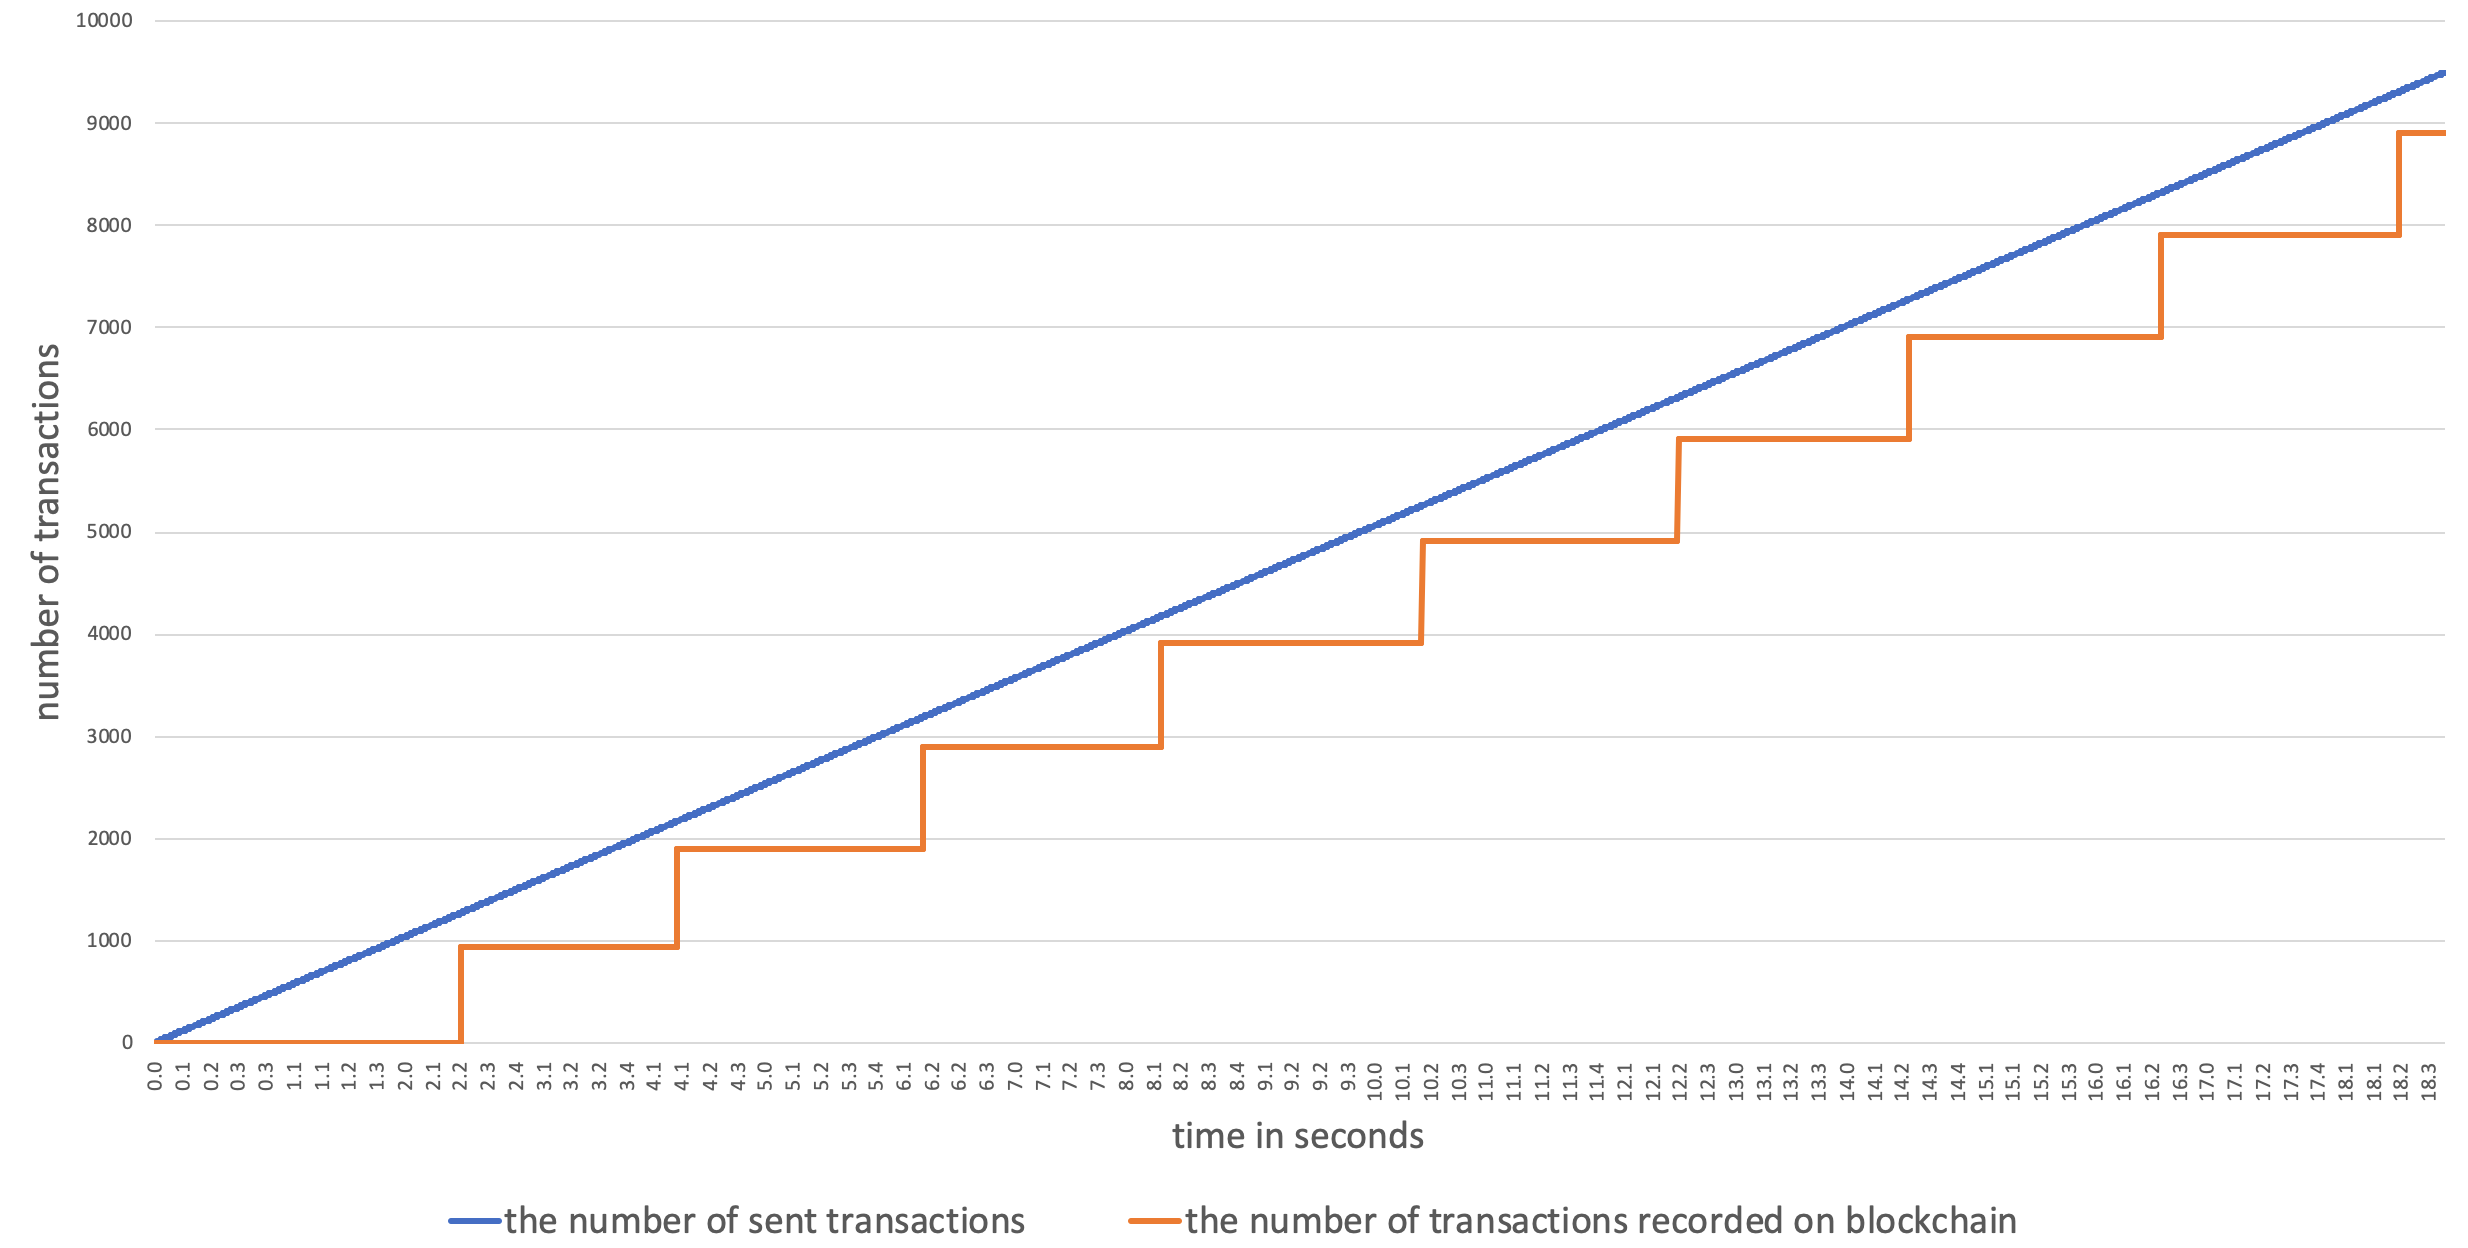
\includegraphics[width=12cm, keepaspectratio]{figures/performance.png}
\caption{Performance Testing}
\label{fig:performance}
\end{figure}

我们在微软云平台上部署了四个区块链节点,每个节点采用标准的D2s v3型号服务器,拥有2 vCPU,2G内存以及1,000 MBps网络带宽。为了测试系统性能,我们生成了1000对公私钥对来模拟1000个用户,每个用户拥有不同的属性,还在随机用户之间生成了10000个随机的授权操作,用于模拟现实中的授权行为。

测试授权数据以每秒500个授权的速率发送给4个节点,区块链网络在大概21秒的时间里成功处理了这些请求。发送的分布时间如图\ref{fig:performance}所示。该网络每2秒生成一个新区块,并且每个区块最多包含1000个授权请求(这一限制设置在代码中)。每个区块包含的授权信息数量如图\ref{fig:performance}所示。实验证明了该系统可以达到每秒处理500个授权请求并且平均延迟在1秒左右,这说明该框架和协议可以应用于现实场景中。
%!TeXroot=。。/main。tex

\chapter{区块链上隐私保护技术}

在区块链系统的实际使用中,为了保证区块链上记录数据的可溯源、可验证等特性,所有数据都必须公开给区块链网络中的所有节点。这一特性在保障安全、可验证的同时,导致恶意攻击者可以直接获取区块链账本中记录的数据,并通过分析数据窥探用户隐私。攻击者通过分析区块链账本中记录的交易数据,发掘其中规律,将用户的不同地址、交易数据关联,并进一步对应到用户的现实身份[7-14]。这类分析攻击主要分为地址聚类和身份定位两阶段。地址聚类阶段根据用户行为特征将可能属于同一用户的地址、交易进行聚类,得到地址间关联关系。身份定位阶段搜集与区块链地址相关联的用户信息,例如论坛、交易所等服务记录的与链上地址对应的手机、邮箱、IP地址等用户链下信息,再根据搜集到的信息确定用户身份,关联该用户所有地址与交易信息,揭露该用户的所有历史记录。

近年来,许多研究者开始关注区块链系统中的隐私问题,该领域中相应的防御技术也不断出现。在区块链隐私分析上,祝烈煌等人从身份隐私和交易隐私两方面分析区块链中的隐私问题,身份隐私指用户身份信息和区块链地址之间的关联关系,交易隐私指区块链中存储的交易记录及背后的知识。Sarah等人提出用抗追溯性来度量区块链中用户信息的匿名性。本文从账本存储和网络通信两个方面,分析区块链系统中隐私信息可能泄露的内容和方式。从账本存储角度,需要保护用户存储在区块链账本上的数据记录所包含的隐私信息;从网络通信角度,需要保护区块链网络中的节点隐私及网络通信中的流量等隐私信息。在隐私保护技术方面,祝烈煌等人[30]从网络层、交易层和应用层出发分别描述区块链隐私保护面临的威胁以及采用的保护技术。Merve等人和李旭东等人将研究分为两大类:基于比特币系统的研究和针对比特币系统进行拓展和替换的研究。

本章对比特币系统以外的区块链隐私保护技术进行更大范围的技术介绍与对比。主要通过技术实现原理,将保护技术划分为地址混淆,信息隐藏和通道隔离,并对各类技术抽象出通用模型,然后介绍各类隐私保护技术的实现及对比。其中地址混淆机制通过交易交换不同用户的资产,对同一用户不同地址间的关联关系进行混淆,从而破坏地址聚类的假设前提;信息隐藏机制通过零知识证明、同态加密等密码学技术加密区块链账本中记录的隐私信息,同时保持账本正确性的可验证;通道隔离机制在区块链网络中设置访问权限,将需要权限访问的数据保护在特定通道中。

\section{区块链隐私及威胁}

传统的区块链系统中通常采用假名机制和广播机制保护用户隐私。其中假名机制指用户可以独立生成任意数量的区块链地址,不需要通过注册或者认证机制。同一用户生成的不同地址可以单独使用,彼此间不存在任何关联关系。因此,仅通过区块链地址无法关联到用户的真实身份,该机制能隔离用户在区块链上不同操作的记录。广播机制指区块链系统通过p2p网络传输数据,网络中采用洪水广播协议传播消息,接受节点无法判断消息来源是消息的直接发起者还是转发者,从而保护消息真实发起者的身份。
假名机制和广播机制能在一定程度上保护区块链用户的隐私安全。但在实际应用中,用户隐私仍面临各类威胁,主要存在于记录数据的分布式账本和区块链去中心化网络中各节点的相关信息。为了保证去中心化系统的正确性和安全性,区块链系统中的所有节点共同维护一致的分布式账本,记录区块链系统中的所有历史数据,用于验证用户提交的新事务的合法性。为了所有节点都能验证账本的正确性,账本中所有数据保持公开,因此账本数据能被攻击者轻易获取,攻击者通过分析公开账本中的记录严重威胁用户隐私。此外,区块链系统采用去中心化网路进行通信,在非许可链系统中,节点加入网络不需要任何身份认证,这在增强了扩展性的同时也导致攻击者可以自由部署节点加入网络,监听网络中各节点隐私信息以及网络中通信信息。本章围绕这两部分介绍需要保护的隐私内容及对应的威胁方式。

\subsection{账本隐私及威胁}

区块链账本记录了区块链系统中的各类事务数据,由于目前区块链系统主要应用于密码货币领域,因此区块链账本主要记录交易数据。交易模型主要分为未花费交易输出(UTXO,UnspentTransactionOutput)模型和账户(Account)模型两类[34]。部分攻击方式针对特定的交易模型,例如交易网络构造攻击和资产追踪攻击针对UTXO模型。账本隐私主要包含以下内容:
交易内容隐私:账本记录的单笔交易内容,包含交易发起方、交易接受方、交易金额以及附带数据等隐私信息。
账户地址隐私:区块链地址与交易的关联关系,包含账户地址的交易记录、账户余额以及不同账户地址间交易关联等隐私信息。
用户身份隐私:用户和区块链地址、交易的关联关系,包含同一用户的交易记录、资金余额等隐私信息。
在区块链系统的实际应用中,用户常需要发起多输入交易,即存在多个输入资产的交易。该交易需要每个输入地址的签名,可以由一个或多个用户生成。由于多个用户对同一交易进行签名的过程较为复杂,通常多输入交易由同一用户生成。此外,在基于UTXO模型的交易系统中,未花费资产只能使用一次,因此当花费资产超过交易所需资产时,用户将超出部分的资产转移到自己的另一账户地址中。用于接受超出部分资产的账户地址通常称为找零地址。针对账本隐私包含的各类隐私,目前的主要攻击方式为账本分析攻击,通过分析区块链账本数据,利用用户常见的交易规律,构建账户地址与交易之间以及用户与账户地址之间的一对多对应关系,威胁账本地址隐私与用户身份隐私。攻击者根据区块链系统的设计与上述使用特征提出以下假设:

\begin{enumerate}
	\item 假设1 多输入交易的所有输入地址为同一用户所持有。
	\item 假设2 交易的找零地址和输入地址为同一用户所持有。
\end{enumerate}

2013年,Reid等人下载了比特币系统2009年1月3日至2011年7月12日的全部账本数据,通过分析数据首先构建交易网络。交易网络中节点表示单次交易,节点间的有向边为交易间的输出-输入对,表示前一次交易的输出作为后一次交易的输入,每条边同时记录了交易金额以及交易时间。

\begin{figure}
\centering
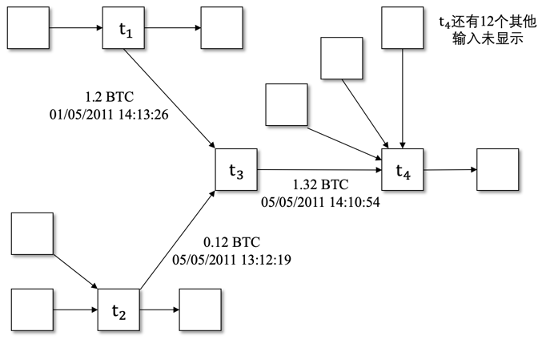
\includegraphics[width=11cm]{figures/sub-network.png}
\caption{交易网络示例}
\label{fig:framework}
\end{figure}

在交易网络的基础上,提取所有多输入交易,构建账户地址间的非完全网络,非完全网络中节点表示地址,节点间有向边表示地址间交易的时间和金额。Reid等人根据中本聪提到的多输入交易关联风险[1]提出假设1,即假设多输入交易的所有输入地址为同一用户所有。基于这一假设,在非完全网络的基础上,可以聚合属于同一用户的所有地址,进而构建用户网络,用户网络中节点表示一个用户,节点间的有向边表示用户间资产流动信息。

(a)Anexamplesub-networkfromtheincompletenetwork
(a)非完全网络中的局部示例

(b)Anexamplesub-networkfromtheusernetwork
(b)用户网络中的局部示例
Fig。2Examplesub-networksfromtheincompletenetworkandtheusernetwork[7]
图2非完全网络与用户网络示例[7]
	2013年,Androulaki等人[8]根据区块链钱包的应用特征提出了挖掘找零地址的方法,如果一个交易拥有两个输出,其中一个为已出现过的地址,另一个为新地址,则将新地址视为找零地址,并提出了假设2,即交易的找零地址和输入地址为同一用户所持有。为了验证假设的正确性,Androulaki等人在大学中构建了模拟的密码货币使用环境,通过搜集用户使用记录,并利用假设1和假设2进行分析,挖掘出40\%左右用户的真实身份。受此启发,Meiklejohn等人[9]给出了“找零地址”更完善的定义:
	找零地址如果交易t中的一个输出公钥地址pk满足以下所有特征,则可将pk视为“找零地址”。
1。	,该地址pk在非完全网络中入度为1,即在区块链账本中首次出现。
2。	交易t为铸币交易以外的普通交易。铸币交易即生成新区块时发布奖励的交易。
3。	不存在且,即不存在“自找零地址”。
4。	不存在,且,即pk为输出地址中唯一首次出现的地址。
综上所述,账本隐私内容主要集中于单次交易的内容及隐藏在多个相关交易之后的用户身份、账户余额等隐私信息。这部分信息记录在公开的区块链账本中,攻击者可以通过分析账本挖掘出其中的关联信息,威胁用户的账本隐私。

\subsection{网络隐私及威胁}

区块链系统通过去中心化的P2P网络进行节点间通信,而在非许可链系统中的网络不存在准入限制,这在增强了扩展性的同时也带来了潜在的风险。攻击者可以任意部署节点,监听网络中各节点隐私信息以及网络通信信息,甚至尝试对正常节点发起攻击。区块链网络主要存在以下隐私内容:

节点隐私:节点自身的隐私内容,包含节点网络IP、软件版本、服务器系统等隐私信息。
通信隐私:节点间通信隐私内容,包含节点间通信的数据内容以及通信流量情况。

2013年,Reid等人尝试利用BitcoinFaucet公开的区块链地址及IP地址对应关系进行分析,揭露比特币用户与实际物理位置的对应关系,该尝试只涉及到很少的节点。Bitnodes网站通过部署大量节点,探测全球范围内的比特币节点信息,其中IP地址分布信息如图3所示(截图于2019年08月01日)。

图3Bitnodes网站在世界范围内发现的比特币节点分布情况

探测攻击严重威胁节点隐私,更进一步,攻击者通过大量探测可以将区块链中广播的数据与实际发起节点关联,尽管区块链网络采用洪水广播的方式保护实际发起人,但是在布置大量探测节点后,攻击者有很大概率找出消息的真实发起节点。2011年,Kaminsky在黑帽大会上提出假设,假设第一次接受到消息时的来源节点即为该消息的真实发起节点。

(a)模式1单一转发者(b)模式2多转发者,无重复转发者


(c)模式3A多转发者,单一重复转发者(d)模式3B多转发者,多重复转发者
Fig。4Fourmessagepropagationmodes
图4四种消息传播模式

2014年,Koshy等人在Kaminsky所提出假设的基础上进行了完善,归纳一段时间内监听到的消息传播情况,提出了区块链网络中消息传播的四种模式(如图4所示)以及对应的真实发起者假设。这一攻击方式通过监听消息传播模式,分析真实发起节点,将IP地址与消息中包含的链上地址对应,威胁通信隐私与用户身份隐私。

模式1单一转发者该模式中消息只有一个节点重复发送。在广播协议中这种情况并不常见,通常出现原因在于该节点发送不合法消息,其他节点拒绝转发该消息。因此可以假设该节点为消息实际发送者。
模式2多转发者,无重复转发者该模式中有多个节点参与消息的转发,每个节点只发送一次。这种模式是网络中最常见的消息传播模式,在Koshy等人收集的数据中占据91。4%。该模式中假设第一次接受到的消息发起者为消息的真实发起者。
模式3A多转发者,单一重复转发者该模式中有多个节点参与消息的转发,除了一个节点重复多次外,其他节点只发送一次。该模式中,假设唯一的重复转发者为消息的真实发起者。
模式3B多转发者,多重复转发者

该模式中有多个节点参与消息的转发,多个节点重复发送,该模式中难以推断实际发起节点,并且所占比例较小,为2。8\%,因此Koshy等人放弃了这部分数据。

综上所述,区块链系统的隐私内容以及对应的攻击方式总结如表2所示。

Table2PrivacyInformationandThreatinBlockchain
表2区块链隐私内容及对应攻击方式

区块链隐私分类	隐私保护内容	隐私威胁攻击方式
交易内容隐私	账本记录的单笔交易信息,包含
交易发起方、交易接受方、交易
金额以及附带数据等隐私信息	通过区块链钱包、浏览器等
工具爬取区块链账本记录
账户地址隐私	区块链地址与交易的关联关系,包
含账户地址的交易记录、余额以及
不同账户间交易等隐私信息	通过分析区块链账本记录,
构建交易网络
用户身份隐私	用户和区块链地址、交易的关联关系,包含同一用户的交易记录、资金余额等隐私信息	利用区块链交易特征,在交易网
络的基础上构建用户网络。也从
论坛、交易所等区块链服务获取
节点隐私	节点相关信息,包含节点网络IP、
软件版本、服务器系统等隐私信息	在区块链网络中部署节点监听
或爬取其他公开信息获取
通信隐私	节点间通信内容,包含节点间通
信的数据内容以及通信流量情况	通过在区块链网络中部署监听节
点,监听节点间通信进行获取

\section{地址混淆机制}

\subsection{中心化混币}

\subsection{去中心化混币}

\section{信息隐藏机制}

\subsection{账本信息隐藏}

\subsection{网络信息隐藏}

\section{通道隔离机制}

\subsection{链下通道隔离}

\subsection{多链通道隔离}


% !TeX root = ../main.tex

\chapter{总结与展望}

\section{全文总结}

访问控制领域是计算机系统中重要的研究领域,直接关系数据的安全和隐私。访问控制模型的发展已经较为成熟,DAC、MAC、RBAC、ABAC等访问控制模型被普遍应用。随着互联网应用的发展,为了提升访问控制的灵活性,OAuth框架广泛用于互联网中向第三方应用提供授权服务。OAuth及类似框架都存在严重中心化的授权服务器,成为系统的性能瓶颈和安全隐患。为了解决这一问题,本文提出采用区块链技术,针对访问控制系统的一些关键技术进行改进和创新,主要贡献如下:

\begin{enumerate}
	\item 针对OAuth框架中存在的中心化授权服务器,提出了区块链网络替代方案,增强系统的安全性和鲁棒性。
	\item 针对区块链账本的存储模式,对基于属性的访问控制系统进行改进,定义符合区块链特点的授权数据结构。
	\item 改进传统的PBFT共识协议,能应用于联盟链的共识过程。
\end{enumerate}

在研究基于区块链技术的访问控制系统的过程中,分布式系统在保障数据安全性的同时,带来了数据泄露的隐私风险。为了保护用户数据在区块链系统中存储和使用的隐私性,本文研究了区块链上隐私保护的技术和实现,将现有的隐私保护技术归纳总结为地址混淆、信息隐藏、通道隔离三大类,并详细介绍了各类隐私保护机制的原理、特征以及不同的实现方式。现有的各类隐私保护机制 及实现技术从不同方面保护区块链隐私,因而在实际考虑隐私保护的区块链系统中,通常综合多种技术达到更全面的隐私保护效果。

\section{未来展望}

基于区块链的访问控制系统未来有广泛的应用场景,但相关研究还较少。本文提出了一些技术的改进,但仍在框架设计、技术细节等方面存在一些需要改进的空间:

\begin{enumerate}
	\item 本文只提出了基于属性的访问控制模型和区块链技术的结合,还需要研究现有其他各访问控制模型基于区块链的实现,增强该系统对现有访问控制系统的兼容性。
	\item 本文采用了改进的PBFT共识协议,该共识协议在性能、扩展性方面还存在不足,难以应用于大型访问控制系统,因此还需要研究其他适用的共识协议。
	\item 本文只研究了现有的区块链上隐私保护技术,还需要改进现有技术使得能应用于访问控制系统中。
\end{enumerate}


% 其它部分
% \backmatter

%% 本科生要求的几个索引。
% \listoffigures    % 插图索引
% \listoftables     % 表格索引
% \listofequations  % 公式索引

% 参考文献
% \bibliographystyle{thuthesis-numeric}      % 顺序编码制
% \bibliographystyle{thuthesis-author-year}  % 著者-出版年制
% \bibliographystyle{thuthesis-bachelor}     % 本科生参考文献的著录格式
% \bibliography{ref/refs}

% 致谢
% \input{data/acknowledgements}

% 声明
% \statement

% 附录
% \appendix
% \input{data/appendix-survey}       % 本科生:外文资料的调研阅读报告
% \input{data/appendix-translation}  % 本科生:外文资料的书面翻译
% \input{data/appendix}

% 个人简历
% % !TeX root = ../main.tex

\begin{resume}

  \resumeitem{个人简历}

  1995 年 07 月 25 日出生于 四川 省 资阳 市。

  2013 年 9 月考入 北京航空航天 大学 计算机科学与技术 系 计算机科学与技术 专业,2017 年 7 月本科毕业并获得 工学 学士学位。

  2017 年 9 月 研究生统一招生考试 进入 清华 大学 计算机科学与技术 系攻读 硕士 学位至今。

  \researchitem{发表的学术论文} % 发表的和录用的合在一起

  % 1. 已经刊载的学术论文(本人是第一作者,或者导师为第一作者本人是第二作者)
  \begin{publications}
    \item Zhang A., Bai X. (2020) Decentralized Authorization and Authentication Based on Consortium Blockchain. In: Zheng Z., Dai HN., Tang M., Chen X. (eds) Blockchain and Trustworthy Systems. BlockSys 2019. Communications in Computer and Information Science, vol 1156. Springer, Singapore (EI 收录, 检索号:20200708163648.)
  \end{publications}

  % 2. 尚未刊载,但已经接到正式录用函的学术论文(本人为第一作者,或者
  %    导师为第一作者本人是第二作者)。
  \begin{publications}[before=\publicationskip,after=\publicationskip]
    \item 张 奥, 白晓颖. 区块链隐私保护研究与实践综述 (已被 软件学报 录用. TH-CPL B类期刊.)
  \end{publications}

  % 3. 其他学术论文。可列出除上述两种情况以外的其他学术论文,但必须是
  %    已经刊载或者收到正式录用函的论文。
  % \begin{publications}
  %   \item Wu X M, Yang Y, Cai J, et al. Measurements of ferroelectric MEMS
  %     microphones. Integrated Ferroelectrics, 2005, 69:417-429. (SCI 收录, 检索号
  %     :896KM)
  %   \item 贾泽, 杨轶, 陈兢, 等. 用于压电和电容微麦克风的体硅腐蚀相关研究. 压电与声
  %     光, 2006, 28(1):117-119. (EI 收录, 检索号:06129773469)
  %   \item 伍晓明, 杨轶, 张宁欣, 等. 基于MEMS技术的集成铁电硅微麦克风. 中国集成电路,
  %     2003, 53:59-61.
  % \end{publications}

  % \researchitem{研究成果} % 有就写,没有就删除
  % \begin{achievements}
  %   \item 任天令, 杨轶, 朱一平, 等. 硅基铁电微声学传感器畴极化区域控制和电极连接的
  %     方法: 中国, CN1602118A. (中国专利公开号)
  %   \item Ren T L, Yang Y, Zhu Y P, et al. Piezoelectric micro acoustic sensor
  %     based on ferroelectric materials: USA, No.11/215, 102. (美国发明专利申请号)
  % \end{achievements}

\end{resume}


% 本科生的综合论文训练记录表
% \includepdf[pages=-]{scan-record.pdf}

\end{document}
